\documentclass[%
 reprint,
superscriptaddress,
%groupedaddress,
%unsortedaddress,
%runinaddress,
%frontmatterverbose, 
%preprint,
%preprintnumbers,
%nofootinbib,
%nobibnotes,
%bibnotes,
 amsmath,amssymb,
 aps,
%pra,
%prb,
%rmp,
%prstab,
%prstper,
%floatfix,
]{revtex4-2}

\usepackage{graphicx}% Include figure files
\usepackage{dcolumn}% Align table columns on decimal point
\usepackage{bm}% bold math
\usepackage{hyperref}% add hypertext capabilities
\usepackage{physics} % for \ket and other quantum notation
\usepackage{amsthm}
%\usepackage[mathlines]{lineno}% Enable numbering of text and display math
%\linenumbers\relax % Commence numbering lines

%\usepackage[showframe,%Uncomment any one of the following lines to test 
%%scale=0.7, marginratio={1:1, 2:3}, ignoreall,% default settings
%%text={7in,10in},centering,
%%margin=1.5in,
%%total={6.5in,8.75in}, top=1.2in, left=0.9in, includefoot,
%%height=10in,a5paper,hmargin={3cm,0.8in},
%]{geometry}
\newtheorem{theorem}{Theorem}[section]
\newtheorem{corollary}{Corollary}[theorem]
\newtheorem{lemma}[theorem]{Lemma}
\newtheorem{definition}{Definition}[section]

\DeclareRobustCommand{\bbone}{\text{\usefont{U}{bbold}{m}{n}1}}

\DeclareMathOperator{\EX}{\mathbb{E}}% expected value

\begin{document}

\preprint{APS/123-QED}

\title{One-way Symmetric Private Information Retrieval Protocol with One Single Database Achieving Statistical Security}% Force line breaks with \\

\author{Xiang Zou}
\email{xiang.zou@mail.utoronto.ca}
\thanks{These authors contributed equally to this work.}
\affiliation{%
 Department of Physics, University of Toronto, 60 St. George Street, Toronto, ON, M5S 1A7, Canada
}

\author{Hoi Fung Chau}
\email{hfchau@hku.hk}
\thanks{These authors contributed equally to this work.}
\affiliation{%
 Department of Physics, The University of Hong Kong, Pokfulam Road, Hong Kong Island, Hong Kong
}%

\date{\today}

\begin{abstract}
Symmetric private information retrieval (SPIR) is an information acquisition target that involves two trusted but curious parties with eavesdroppers, and it has significant theoretical and commercial value, due to that it enables a user to retrieve one item from a database without revealing the query index, while also preventing the user from learning anything beyond the requested item, even with unbounded computation. This paper proposes and investigates the first candidate protocol to single-database SPIR in an information-theoretic setting by using a one-way, prepare-and-measure quantum architecture inspired by BB84 and standard QKD post-processing. We prove the security of the protocol against any third-party eavesdropper, and we show that the asymptotic security against any of the involved parties cheating. The proposed protocol has great interest in numerous real-life applications, including official investigations, and it enhances our understanding of the limits of quantum cryptography.
\end{abstract}


\keywords{Symmetric Private Information Retrieval, Quantum Key Distribution, Quantum Cryptography}%Use showkeys class option if keyword%display desired
\maketitle

%\tableofcontents

\section{Introduction}

Secure access to remote databases is a central primitive in both classical and quantum cryptography~\cite{QPQ1, QPQ2, QPQ3, QSPIR_multiple_database1, QSPIR_multiple_database2, Insecurity_Quantum_Oblivious_transfer1}, with applications ranging from cloud storage and biometric identification to distributed ledgers and secure multiparty computation. In this context, private information retrieval (PIR) allows a client to retrieve partial data from a database held by a server without revealing which item was requested, thereby protecting the privacy of the client’s query. While Symmetric private information retrieval (SPIR) strengthens this notion by additionally requiring database privacy, the client must not learn anything about the database beyond the requested item, even if the client is computationally unbounded~\cite{QSPIR_theory1, QSPIR_multiple_database1, QSPIR_multiple_database2, SPIR1, SPIR2, SPIR3}.

Classical PIR and SPIR have been extensively studied before~\cite{PIR1, PIR2, PIR3, SPIR1, SPIR2, SPIR3}. In the information-theoretic setting, it is by now well understood that single-server PIR and SPIR suffer from strong limitations in classical communication: if only one database server is available and no computational assumptions are made, then any PIR scheme with perfect user privacy must reveal essentially the entire database to the user, and information-theoretic SPIR with a single database server is impossible except for the trivial protocol where the entire database is sent~\cite{PIR1, PIR2}.


To obtain nontrivial communication complexity and database privacy, classical SPIR protocols assume either multiple non-communicating database servers that share randomness, or they rely on computational hardness assumptions such as the hardness of lattice or number-theoretic problems~\cite{SPIR1, SPIR2, SPIR3}.

These multi-server SPIR protocols can achieve sublinear communication complexity~\cite{SPIR1, SPIR2, SPIR3} and strong security guarantees, but they require architectural assumptions—such as multiple independent data centers and pre-distributed shared randomness—that may be difficult or costly to realize in practice, if not impossible.

Quantum communication offers new tools to revisit PIR and SPIR. Genuinely quantum protocols can outperform classical ones in certain regimes: for example, quantum symmetrically-private information retrieval (QSPIR) schemes achieve sublinear communication with multiple servers and no shared randomness~\cite{QSPIR_multiple_database1, QSPIR_multiple_database2}, while still protecting both user and database privacy against honest-but-curious participants.

A parallel line of work on quantum private queries (QPQ) has proposed cheat-sensitive protocols~\cite{QPQ1, QPQ2, QPQ3} in which a single quantum server can answer private queries to a classical database with strong user privacy and bounded database leakage per query, at the price of relaxing full information-theoretic guarantees and allowing detection of server misbehaviour instead of preventing a third-party eavesdropper.

More recently, quantum-key-distribution (QKD)-assisted SPIR protocols and experimental demonstrations~\cite{QSPIR_multiple_database1, QSPIR_multiple_database2} have shown that quantum networks can be leveraged to distribute the secret keys and shared randomness needed for multi-database SPIR, but these schemes still fundamentally rely on multiple non-colluding databases or trust in specific network assumptions.

Despite this progress, the status of fully symmetric, information-theoretic private information retrieval from a single classical database remains unclear in the quantum setting. Existing negative results show that, under natural correctness and privacy requirements, perfect single-database SPIR is impossible even when quantum communication is allowed~\cite{Insecurity_Quantum_Oblivious_transfer1}, mirroring the classical impossibility of information-theoretic single-server SPIR.

In this work, a one-way quantum-communication protocol is presented that realizes symmetric private information retrieval between a single client and a single classical database server in an information-theoretic setting with statistical security.
The protocol uses a prepare-and-measure QKD-type architecture in which Alice, with a database, sends single-photon polarization states drawn from the BB84 alphabet to Bob, who is interested in parts of the database, over a one-way quantum channel, followed by classical post-processing over an authenticated classical public channel.

Operationally, the proposed protocol is attractive in that it uses only standard BB84-type sources and measurements, together with classical permutation, error correction, and privacy amplification, all of which are well within the reach of current QKD technology~\cite{Experimental_QKD1}. The one-way nature of the quantum communication, together with the fact that only a single database server is required, makes the architecture conceptually simple and directly compatible with existing quantum-communication links between a client and a data center.

This work thus provides a concrete candidate for achieving SPIR with one client, one classical database, and one-way quantum communication, together with explicit resource trade-offs between the database size, the block length, the unambiguous discrimination success probability, and the tolerated quantum bit error rate.

\section{Problem Statement and Definition}
\label{sec:formal_definition}

Suppose there are two mutually trusted but curious parties, Alice and Bob, with access to both classical and quantum communication channels, which are completely controlled by an all-powerful eavesdropper, Eve. Let $\Sigma=\{0, 1\}$. Suppose Alice holds a bit-string, the database, $\textbf{d}=\{d_0, d_1, \cdots, d_n\}\in\Sigma^n$ from an distribution $X$, and Bob is interested in bit $i$.

We will demonstrate the existence of a class of SPIR protocol with statistical security that utilizes a one-way quantum channel from Alice to Bob, along with public broadcasting channels accessible to both Alice and Bob. Upon the completion of the protocol, Bob will obtain a bit-string $\mathbf{y} \in \{0, 1\}^n$, Eve will obtain a bit-string with her control over the channels \( \mathbf{w} = \{w_0, w_1, \cdots, w_n\} \in \{0, 1\}^n \), and Alice will guess the index $i$, denoted by $i'$ of the database $\mathbf{d}$ that Bob wanted.

By employing some additional resources, the protocol will be largely similar to a QKD setup. After the protocol, we require that this SPIR protocol is $\epsilon_{sec}$-secret. To define the secrecy of a key, we consider the quantum state $\rho_{BE}$ that describes the correlation between Alice’s classical key $\mathbf{s_b}$ and the eavesdropper, $E$ (for any given attack strategy). A key is called $\Delta$-secret from $E$ if it is $\Delta$-close to a uniformly distributed key that is uncorrelated with the eavesdropper, that is, if

\begin{equation}
    \min_{\sigma_E}\frac{1}{2}\norm{\rho_{BE}-\omega_B\otimes\sigma_E}_1\le\Delta
\end{equation}

Where $\omega_B$ denotes the maximally mixed state held by Alice. Then, a protocol is called $\epsilon_{sec}$-secret if the protocol outputs $\Delta$-secret keys, such that
\begin{equation}
    (1-p_{abort})\Delta \le\epsilon_{sec}
\end{equation}
Where $p_{abort}$ is the probability of the protocol being aborted. Therefore, the success of our protocol is parametrized by 2 parameters, $p_{fail}$ corresponds to the probability that Bob gains more information than expected, while $\epsilon_{sec}$ characterizes the information on Alice's database gained by the eavesdropper.

Meanwhile, the protocol is $\epsilon_{cor}$-correct for the bit-string $\mathbf{y}$ obtained by Bob, meaning that \(\Pr[y_i \ne d_i] \le \epsilon_{cor} \). Additionally, denote the remaining bit strings \( \mathbf{d'} = \{d_0, \cdots, d_{i-1}, d_{i+1}, \cdots, d_n\} \) and \( \mathbf{y'} = \{y_0, \cdots, y_{i-1}, y_{i+1}, \cdots, y_n\} \), we require that $\mathbf{d'}$ is $\epsilon_{A}$-secret to $\mathbf{y'}$ with the same definition as above. This ensures that Bob gains no information about Alice beyond the specific bit of interest asymptotically.

Last but not least, we require that $\Pr[i'=i]=1/n+\epsilon_{guess}$ for some small number $\epsilon_{guess}$, meaning that the guess index from Alice is not much better than a random guess.

To summarize in simple terms, upon completion of this protocol, if all three of the following criteria are met, the protocol is considered implemented successfully, in descending priority.
\begin{enumerate}
    \item No information is leaked to Eve.

    \item Alice has no idea which bit of information Bob wants.

    \item Bob can only get the bits of information he wants.
\end{enumerate}

We have made the following central assumptions:
\begin{enumerate}
    \item Bob has no long-term quantum memory.  
\end{enumerate}

\section{The Protocol}
\label{sec:the_protocol}
In this section, we will describe the protocol that Alice and Bob use to achieve SPIR. The quantitative analysis will be discussed in later sections. This work is inspired of different well-studied QKD protocols in the prepare and measure scheme, where Alice prepares one of the four states, $\ket{0}, \ket{1}, \ket{+}, \ket{-}$, in photonic set up, it may represent the 4 polarizations of the photons, Horizontal, Vertical, Diagonal, and Anti-diagonal, respectively. Whereby convention, $\ket{0}, \ket{+}$ represent the physical bits $0$ in the $\sigma_Z$ and $\sigma_X$ basis respectively with a $+1$ eigenvalue; then, $\ket{1}, \ket{-}$ represent the physical bits $1$ in their respective basis with a $-1$ eigenvalue, for notational simplicity, we will use $X$-basis and $Z$-basis.

Alice holds a database of $n$ bits of data. Alice and Bob will collectively come up with an integer $k$, where they aim at achieving a length $(kn)$ of physical bits at the end. The reason for needing the parameter $k$ will be clear in step 7. Meanwhile, they will agree on 2 other integers $m$ and $h'$; their usage will be explained later. 

\begin{definition}[\textbf{The SPIR Protocol}]
    We define a family of SPIR protocols, $SPIR(n, k, m, h, e_{thr}, \epsilon_{cor}, \epsilon_{A}, \epsilon_{B}, \text{leak}_{EC})$, which is parametrized by the size of the database $n$, an integer $k$ corresponding to the block size (will be introduced later). Number of bits used for parameter estimation, $m$. A required pre-shared secret key between Alice and Bob of length $h$. The quantum channel threshold error rate $e_{thr}$. The correction leakage $\epsilon_{cor}$. Apart from the intended bit, Bob's remaining bit-string is $\epsilon_A$-secret to the database held by Alice, $\epsilon_B$ is the upper-bound of the probability of Alice guessing the index of Bob's interested bit compared to a random guess, and the error correction leakage, $\text{leak}_{EC}$.
\end{definition}

In our setting, the two parties, Alice and Bob, are honest but curious, while their primary target is that any eavesdropper, Eve, who gains the least amount of information from their communication. Later, we will see that after the protocol, Alice will obtain a secret key $\mathbf{s_b}$ of length $n$, and use it to encode the database $\mathbf{d}$.

\begin{enumerate}

    \item Alice randomly prepares one of the four states, $\ket{0}, \ket{1}, \ket{+}, \ket{-}$, and sends it to Bob. Bob acknowledges receipt and chooses a random basis (either $\sigma_Z$ or $\sigma_X$) to measure the state. Bob marks down both the chosen basis and the measurement result. The process is repeated until $kn+m+h'$ qubits are received by Bob, then Alice will wait for sufficiently long, until we have confidence to say that the coherence time of the quantum memory used by Bob expires. 

    \item Alice and Bob use $m$ received states to estimate the error, where Alice picks $m$ states and notifies Bob, and Bob will publicly announce the measurement basis and result, and then, Alice estimates both the bit flip and phase flip errors that occurred in the channel; if the error rate is too high, they abort the protocol; otherwise, they proceed. Then, they calculate the QKD key rate, denoted by $r$.

    \item For the remaining $kn+h'$ states, they will use $h'$ qubits to perform a normal QKD process (i.e., publicly announce the basis and discard the mismatched ones, and have a raw key of length $h$, then do error-correction and privacy amplification with some pre-shared privacy). Then they obtain a shared private key of length $hr$. These $hr$ bits private key are used for padding for the error-correction code in later stages; theoretical analysis in Section~\ref{sec:QECC_existence}. 

    \item For the remaining $kn$ states, Alice will reveal partial information about that state. For example, if Alice prepared $\ket{0}$ or $\ket{-}$, it classically announces that ``the state he prepared is either $\ket{0}$ or $\ket{-}$". Similarly, if either $\ket{1}$ or $\ket{+}$ was prepared, it classically announces that ``the state it prepared is either $\ket{+}$ or $\ket{1}$''. 

    \item Following the Unambiguous State Discrimination (USD). For each state, with probability $b$, Bob can unambiguously determine the state, whereas with a probability $(1-b)$, Bob cannot. Here, $b$ represents the probability of USD, theoretical noiseless maximum $b = 1-\norm{\bra{0}\ket{-}} = 1-\norm{\bra{1}\ket{+}} \approx 0.293$. If Bob can unambiguously determine the state, Bob marks it as "unambiguous" and records the physical bits. Otherwise, Bob marks down "ambiguous" and 0 or 1 randomly.

    \item By now, Alice and Bob have shared an imperfect bit-string of length $kn$. Denote the bit string held by Alice as $\mathbf{s_b}$, and that by Bob as $\mathbf{s_a}$; both bit strings are indexed. Denote the index sting to be $\mathbf{s'}=\langle1, 2, 3, \cdots, kn\rangle$.

    \item Alice randomly permutes the bit string $\mathbf{s_b}$, and partition them into $n$ blocks separately, denoted as $\mathbf{s_{b1}}, \mathbf{s_{b2}},\cdots \mathbf{s_{bn}}$, and each block has $k$ bits, that $\mathbf{s_b}=\cup_i \mathbf{s_{bi}}$ Furthermore, we note down the indices of each bit in every block in the original bit-string $\mathbf{s_b}$, and denote it as $\mathbf{s_{1}'}, \mathbf{s_{2}'},\cdots \mathbf{s_{n}'}$.

    \item Alice will publicly announce the index strings $\mathbf{s_1'}, \mathbf{s_2'},\cdots \mathbf{s_n'}$. And ask for a permutation from Bob. Meanwhile, Alice and Bob will choose a $[[k, 1, d]]$ quantum error correction code for $d=\frac{(1-b-\epsilon)}{1+e}k$. $e$ is the quantum channel error rate and $\epsilon$ is some user-defined threshold. Explanation and analysis of each parameter are discussed in Section~\ref{sec:QECC_existence}.

    \item After receiving the $n$ index strings $\mathbf{s_1'}, \mathbf{s_2'},\cdots \mathbf{s_n'}$ and knowing the QECC code that they agreed on, Bob knows which block is correctable. If Bob found that no blocks are correctable, she will simply ask Alice to re-shuffle and rearrange the qubits into another set of blocks. The process is repeated until Bob has one block that is correctable. 
    
    \item Bob will arrange the $n$ index strings and place the correctable block in the relevant bit, and then return the permuted index strings to Alice. For example, Alice has a database of 5 bits, hence there are 5 blocks of $k$ bits. Suppose Bob can only correct the $2^{nd}$ block, and she is interested in the $5^{th}$ bit, then she may return a permuted block to Alice as $3, 5, 4, 1, 2$. The key here is that block $2$ is placed at location $5$. 

    \item Upon receiving the permuted index strings, Alice applies the QEC code to each block $\mathbf{s_{b1}}, \mathbf{s_{b2}},\cdots \mathbf{s_{bn}}$, and obtains an $n$-bit shifting key $\mathbf{s_s}\in\Sigma^n$. Then, Alice sends to Bob $\mathbf{y}=\mathbf{d}\oplus\mathbf{s_s}$, where $\mathbf{d}$ represents the database.

    \item Bob will apply the QEC code to the block that is correctable and obtain a single-bit shifting key $s_s'$, and upon receiving $\mathbf{y}$ from Alice, suppose she is interested in the $i^{th}$ bit, she will select the $y_i$ that she is interested in and get back $d_i=y_i\oplus s_s'$.
    
\end{enumerate}

Our protocol is very similar to the classic BB84 protocol for Quantum Key Distribution, except for several crucial modifications.

\begin{enumerate}
    \item In step 1, after Alice sends out the satets, she waited for sufficiently long, to ensure Bob's Quantum memory expires. This prevents Bob's cheating strategy by delaying measurement.
    
    \item In step 2, the error estimation ensures that the eavesdropper gains asymptotically no information; a theoretical analysis is presented in Section~\ref {sec:Review_qkd_security}. The error estimation step is entirely done by Alice, this prevents Bob's cheating strategy by measuring in bases other than $\sigma_X$ and $\sigma_Z$.
\end{enumerate}

\subsection{Intuitional Understanding of the Protocol}

Here, we provide an intuitive explanation of why the protocol works. Alice has a database $\mathbf{d}$ of length $n$, and Bob is interested in the $i$-th bit. The protocol works as follows: Alice and Bob will first perform close to the normal QKD procedures to ensure the channel error rate is low enough and obtain a long enough string of shared qubits. They will use part of this string to perform sifting and error correction to obtain a private key.

For the rest of the qubits, Alice and Bob perform the USD protocol, where Alice and Bob have a shared erroneous string $\mathbf{\ell}_A$ and $\mathbf{\ell}_B$ of length $kn$ respectively, that $\mathbf{\ell}_A$ and $\mathbf{\ell}_B$ are certainly agreed on statistically $\approx bkn$ bits, recall that $b$ is the success rate of USD. The difference being, Bob knows which $\approx bkn$ bits are agreed between $\mathbf{\ell}_A$ and $\mathbf{\ell}_B$, while Alice does not know that.

Then, Alice will randomly arrange the string into $n$ blocks, and each block has $k$ bits. Statistically speaking, for each block, Bob knows $\approx bk$ bits out of the $k$ bits. The number of bits Bob knows about each block follows a Gaussian distribution $\mathcal{N}(bk, \sigma)$ for some variance $\sigma^2$, which depends on $k, b$ and some other parameters. Detailed quantitative analysis is in Section~\ref{sec:Bob_Cheating}. Consequently, with some of the blocks, Bob knows $> bk$ bits, and for some blocks, Bob knows $\le bk$ bits.

When Alice chooses a QECC, Alice chooses one that corrects $[[k, 1, 1-b(k-\epsilon)]]$ bits, with a small number $\epsilon$ determined by Alice. We will show in Section~\ref{sec:QECC_existence} that under certain conditions of the channel, such QECC always exist. So, for most of the blocks, Bob cannot correctly distill a bit. While ideally, for 1 block, Bob can distill a single bit based on statistical arguments, detailed theoretical analysis is in Section~\ref{sec:Bob_Cheating}.

Then, Alice and Bob apply the QECC to all $n$ blocks, and distill a string $\mathbf{s_s}$ of $n$ bits. Here, ideally, Bob only knows 1 bit from this string with certainty, and Bob will send Alice a permutation pattern of this bit string where Bob puts the index of the bit she knows to the $i$-th place, and Alice returns $\mathbf{d}\oplus \mathbf{s_s}$, where Bob can get the bit she wants.

\section{Security Against Eve}

We have briefly reviewed the security proof, asymptotic, and finite key rate of the QKD protocols in Appendix~\ref{sec:Review_qkd_security}, we will show that the same techniques are also applicable to our SPIR protocol to ensure no information is leaked to Eve. Hence, in this section, we will show that there exists an $SPIR(n, k, m, h, e_{thr}, \epsilon_{cor}, \epsilon_{A}, \epsilon_{B}, \text{leak}_{EC})$ protocol that is $\epsilon_{sec}$-secret against Eve.

As an aside, in Appendix~\ref{sec:Depolarizing_and_Dephasing_Noise}, we will discuss the two common types of errors, the depolarizing and dephasing errors, and show how the channel error rate $e$ is related to the depolarizing and dephasing strengths.

\subsection{The Existence of the QEC Code Against Eve}
\label{sec:QECC_existence}
Multiple previous results on the security of QKD~\cite{Shor_Preskill_Proof1} have shown that by performing Error Correction and Privacy Amplification, or equivalently applying a one-way QEC code, the protocol can be made $\epsilon_{sec}$-secret against Eve. The requirement here is such QEC code exists. In this subsection, we will focus on the theoretical infinite-key analysis, and in the next subsection, the finite key effect will be considered.

In our setup, the fundamental problem is whether such $[[k, 1, d]]$ QEC code exists for $d=\frac{(1-b-\epsilon)}{1+e}k$ or not. Will it break some well-established bounds for QEC code? Unfortunately, the answer is yes. As demonstrated in Shor and Preskill's proof, the prepare and measure QKD with privacy amplification is equivalent to a one-way entanglement-distillation process. Thus, the prepare-and-measure QKD with privacy amplification is equivalent to a QEC code $[[n, \lfloor rn\rfloor, \lfloor en\rfloor]]$, where $r$ is the channel key rate, and $e$ is the channel error rate. And the key rate is given by:
\begin{equation}
    r\le 1-2H_2(e)
\end{equation}
For $H_2(e)$ representing the binary entropy function.

In order to find a $[[k, 1,\frac{(1-b-\epsilon)}{1+e}k]]$ QEC code, we have the block key rate $r'=1/k$ and the block error rate $e'=\frac{(1-b-\epsilon)}{1+e}$. While this is impossible, as almost certainly $e'$ will be big enough to break the Quantum Hamming Bound for finite-length codes. Luckily, there's a way to rescue it. Remember in step 3 of the protocol in Section~\ref{sec:the_protocol}, Alice sent $h'$ extra states to Bob, where they perform a normal QKD process and got a shared-private key of length $hr$. Then, Alice distributes these $hr$ private bits to the $n$ blocks, and each block now contains $k+hr/n$ bits, and now the problem becomes to find a $[[k+hr, 1, \frac{(1-b-\epsilon)}{1+e}k]]$ QEC code. Denotes that the block key rate $r'$ and block error rate $e'$ for each block are (recall that $e$ is the channel error rate and $r$ is the Shor-Preskill key rate of the BB84 QKD scheme):
\begin{equation}
    e'=\frac{(1-b-\epsilon)k}{(k+hr/n)(1+e)}, \quad r'=\frac{1}{k+hr/n}
\end{equation}

Here, remark that the block key rate $r'$ and block error rate $e'$ do not necessarily need to follow the Shor-Preskill key rate bound, i.e., $r\le 1-H_2(e)$, as this bound is to ensure that the underlying QKD protocol is secure against Eve, meaning that asymptotically, Eve can gain no information from Alice and Bob. Therefore, in the first stage, when Alice and Bob estimated the channel error rate and apply error correction and privacy amplification, it satisfies $kr\ge k(1-H_2(e))\ge1$, then the protocol is already safe against Eve. The block error rate is to ensure that there exists such CSS code where Bob can decode a bit from the correctable block.

The block error rate depends on the extra resources $h$, so there exists some $h$, $[[k+hr/n, 1, \frac{(1-b-\epsilon)}{1+e}k]]$, which we have left to do is to find $h$, such that a CSS QEC code exists within the Quantum Gilbert-Varshamov Bound.

Recall that the Quantum Gilbert-Varshamov Bound proves the existence of a stabilizer code through a constructive, probabilistic mathematical argument. It guarantees that an $[[n, k, d]]$ stabilizer code exists if 
\begin{equation}
    \sum_{j=0}^{d-1}\binom{n}{j}3^j <2^{n-k}
\end{equation}

Substituting our parameters into the above bound, a stabilizer QEC code $[[k+hr, 1, \frac{(1-b-\epsilon)}{1+e}k]]$ exists for each block if

\begin{equation}
    \sum_{j=0}^{\frac{(1-b-\epsilon)}{1+e}k-1}\binom{k+hr/n}{j}3^j <2^{k+hr/n-1}
\end{equation}

Solving the above inequality will yield that $h\ge f(n, k, r, b,\epsilon)$ for a very complicated function $f$, which gives a lower bound on the overhead needed to make this protocol work. However, the above inequality is, in general, very hard, if not impossible, to solve; instead, we now try to approximate it.

Let $\text{Vol}_q(n, \alpha n)$ denote the volume of a $q$-ary Hamming ball of radius $\alpha n$, where $0 \le \alpha \le 1 - 1/q$ and $\alpha n$ is an integer. The volume is bounded both above and below by the $q$-ary entropy function:

\begin{equation}
    \text{Vol}_q(n, \alpha n) = \sum_{j=0}^{\alpha n} \binom{n}{j}(q-1)^j
\end{equation}

The standard asymptotic upper bound is:
\begin{equation}
    \sum_{j=0}^{\alpha n} \binom{n}{j}(q-1)^j \;\leq\; q^{\,n\,H_q(\alpha)}
\end{equation}

For a sharper estimate of its lower bound, applying Stirling's approximation to the binomial coefficient yields a tighter prefactor:
\begin{equation}
    \sum_{j=0}^{\alpha n} \binom{n}{j}(q-1)^j \;\geq\; \frac{1}{\sqrt{8 n \alpha(1-\alpha)}} \, q^{\,n\,H_q(\alpha)}
\end{equation}

In our case, $q=4$ for the QEC code, with $\alpha = \frac{L}{k + hr/n}$ and $L=\frac{(1-b-\epsilon)}{1+e}k-1$,

\begin{equation}
    \frac{4^{(k + hr/n) H_4(\alpha)}}{\sqrt{8 (k+hr/n) \alpha(1-\alpha)}}\le\sum_{j=0}^{L} \binom{k + hr/n}{j} 3^j \leq 4^{(k + hr/n) H_4(\alpha)}
\end{equation}

Hence, the inequality we tried to solve can be rewritten as:
\begin{equation}
\begin{split}
    2^{k+hr/n-1}&>\frac{4^{(k + hr/n) H_4(\alpha)}}{\sqrt{8 (k+hr/n) \alpha(1-\alpha)}}\\
    &>2^{2(k + hr/n) H_4(\alpha)-\log_2{\sqrt{8 (k+hr/n) \alpha(1-\alpha)}}}
\end{split}
\end{equation}
Which simplifies to:
\begin{equation}
\begin{split}
    k+hr/n-1&>{2(k + hr/n) H_4(\alpha)} \\ &\quad-\log_2{\sqrt{8 (k+hr/n) \alpha(1-\alpha)}}\\
    2(k+hr/n)H_4(\alpha)&<k+hr/n \\ &\quad+\log_2{\sqrt{8 (k+hr/n) \alpha(1-\alpha)}}-1\\
    H_4(\alpha)&<\frac{1}{2}+\frac{\log_2{\sqrt{8 (k+hr/n) \alpha(1-\alpha)}}-1}{2(k+hr/n)}
\end{split}
\end{equation}

the right-hand side depends on $\alpha$, which attains maximum when $\alpha=0.5$, hence, we can further simplify the approximate inequality:

\begin{equation}
\begin{split}
    H_4(\alpha)&<\frac{1}{2}+\frac{\log_2{\sqrt{2 (k+hr/n)}}-1}{2(k+hr/n)}\\
    H_4(\alpha)&<\frac{1}{2}+\frac{\log_2\left(\frac{k+hr/n}{2}\right)}{4(k+hr/n)}
\end{split}
\end{equation}

Recall that, in our setting, $k+hr/n$ is the number of qubits used in each block, which is typically very large. Thus, $k+hr/n \gg 1$, hence, $\frac{\log_2\left(\frac{k+hr/n}{2}\right)}{4(k+hr/n)}\ll 1$. For approximation purposes, we can safely drop this term. Here, we have,

\begin{equation}
\begin{split}
    H_4(x) &= x\log_4(3)-x\log_4(x)-(1-x)\log_4(1-x)\\
    &=\frac{x \log_2(3) + H_2(x)}{2}.
\end{split}
\end{equation}

Thus, we have $H_4(\alpha)<1/2$,
\begin{equation}
    \alpha\log_2(3)+H_2(\alpha)<1
\end{equation}
By using numerical calculation, we find that the supremum of $\alpha$ is given by:
\begin{equation}
    \alpha^*\approx0.1893
\end{equation}
Substituting $\alpha = L/(k+hr/n)$, and $L=\frac{(1-b-\epsilon)}{1+e}k-1$, and the condition that $\alpha < \alpha^*$ we obtain:
\begin{equation}
    \frac{\frac{(1-b-\epsilon)}{1+e}k-1}{k+hr/n}<\alpha^*
\end{equation}
Which gives a lower bound on $h$:
\begin{equation}
    h>\frac{n(1-b-\epsilon)k}{r(1+e)\alpha^*}-\frac{nk}{r}-\frac{n}{r\alpha^*}
\end{equation}

Now, we will state and prove the full theorem for the walking theorem~\ref{thm:walking_theorem}

\begin{theorem}
    For any channel qubit error rate $e<e_{thr}$, where $e_{thr}$ is the threshold qubit error rate of the QKD protocol used, the presented SPIR protocol in Section~\ref{sec:the_protocol} can be achieved with an overhead $h$ of
    \begin{equation}
        h>\frac{n(1-b-\epsilon)k}{r(1+e)\alpha^*}-\frac{nk}{r}-\frac{n}{r\alpha^*}
    \end{equation} 
    qubits, where $n$ is the length of Alice's database, $k$ is the number of qubits per block, $b$ is the success probability of the unambiguous state discrimination, and $\epsilon$ is some arbitrary number to adjust the probability of Bob cheating.
\label{thm:success_protocol}
\end{theorem}

\begin{proof}
    The protocol success means $\exists h, s.t. [[k+hr/n, 1, d]]$ exists, for $d=\frac{(1-b-\epsilon)}{1+e}k$ and $r\le1-2H_2(e)$. In the above section, we have shown that when the quantum GV bound is satisfied, we must be able to find a QEC code that satisfies the parameters.

    Through simple calculation and estimation, we obtain,
    \begin{equation}
         h>\frac{n(1-b-\epsilon)k}{r(1+e)\alpha^*}-\frac{nk}{r}-\frac{n}{r\alpha^*}
    \end{equation}
    The right-hand side of the above inequality has poles only at $e\rightarrow-1^+$ and $r=0$. Since, $e>0$. The only realistic pole is at $r=0$. As $r\ge0$, which means the channel error rate is lower than the channel threshold error rate $e<e_{thr}$, we can always find a lower bound for the equation of $h$. Hence, we have proven that $\forall e<e_{thr}, \exists h, s.t.,$ the protocol can succeed.
\end{proof}

Shor and Preskill's proof is based on CSS-type QEC codes, which can be thought of as a combination of 2 classical codes, one correcting bit-flip error and the other correcting phase flip error~\cite{CSS_Shor_Calderbank, CSS_Steane, Shors_9_qubits_code}. For example, Alice can choose some Topological QEC codes, as they have currently received great experimental success~\cite{Surfacecode1, google_surface_code, TQEC1}

\subsection{Finite-Key Analysis}
When considering finite-key analysis and the application of real codes, that changes our overhead estimation $h$ in Theorem~\ref{thm:success_protocol}.

However, in Section~\ref{sec:QECC_existence}, we discussed the existence of a QECC that achieves our protocol, making assumptions about the asymptotic key rates, particularly the resource overhead $h$, as stated in Theorem~\ref{thm:success_protocol}. Everything that needs to be modified in a finite-key setting is the finite-key key rate $r_{real}$, and the corresponding finite-key threshold error rate $e_{thr}^{real}$.

Recall that in Section~\ref{sec:Finite_key_analysis_qkd}, we presented an approximate realistic key rate as in Equation~\ref{eq:realistic_rate}, followed by previous literature Ref.~\cite{Rates_for_realistic_code1, Rates_for_realistic_code2, Rates_for_realistic_code3, Finite_key_analysis1, Finite_key_analysis2, Finite_key_analysis3}, where we adopt our convention, that $n$ is the length of Alice's database, and $k$ is the block length for QEC agreed by Alice and Bob.

\begin{equation}
    r_{real}\approx (q-H(e_{tol}+\mu)-1.16H(e_{tol}))/c-\frac{\log_2 \frac{2}{\epsilon_{sec}^2\epsilon_{cor}}}{nkc}\\
    \label{eq:realistic_rate}
\end{equation}

The new threshold error rate can be calculated by setting
\begin{equation}
    r_{real}>0
\end{equation}
Solving this very complicated equation will reveal us $e_{thr}^{real} = f(\Phi[n, m, l, e_{tol}, \epsilon_{cor}, \epsilon_A, \epsilon_B \text{leak}_{EC}], q, \epsilon_{sec})$. However, solving this equation is again extremely hard, if not impossible; and here we try to get reasonable bounds for $e_{thr}^{real}$, assuming $m=\sqrt{n}$, meaning that the number of qubits used for parameter estimation scales as the square root of $n$, which is reasonable~\cite{Finite_key_analysis1, Finite_key_analysis2, Finite_key_analysis3}.

\begin{equation}
    \begin{split}
        nk(q-H(e_{thr}^{real}+\mu)-1.16H(e_{thr}^{real}))&>\log_2 \frac{2}{\epsilon_{sec}^2\epsilon_{cor}}\\
        H(e_{thr}^{real}+\mu)+1.16H(e_{thr}^{real})&<q-\frac{1}{nk}\log_2 \frac{2}{\epsilon_{sec}^2\epsilon_{cor}}\\
    \end{split}
\end{equation}

\begin{figure}
    \centering
    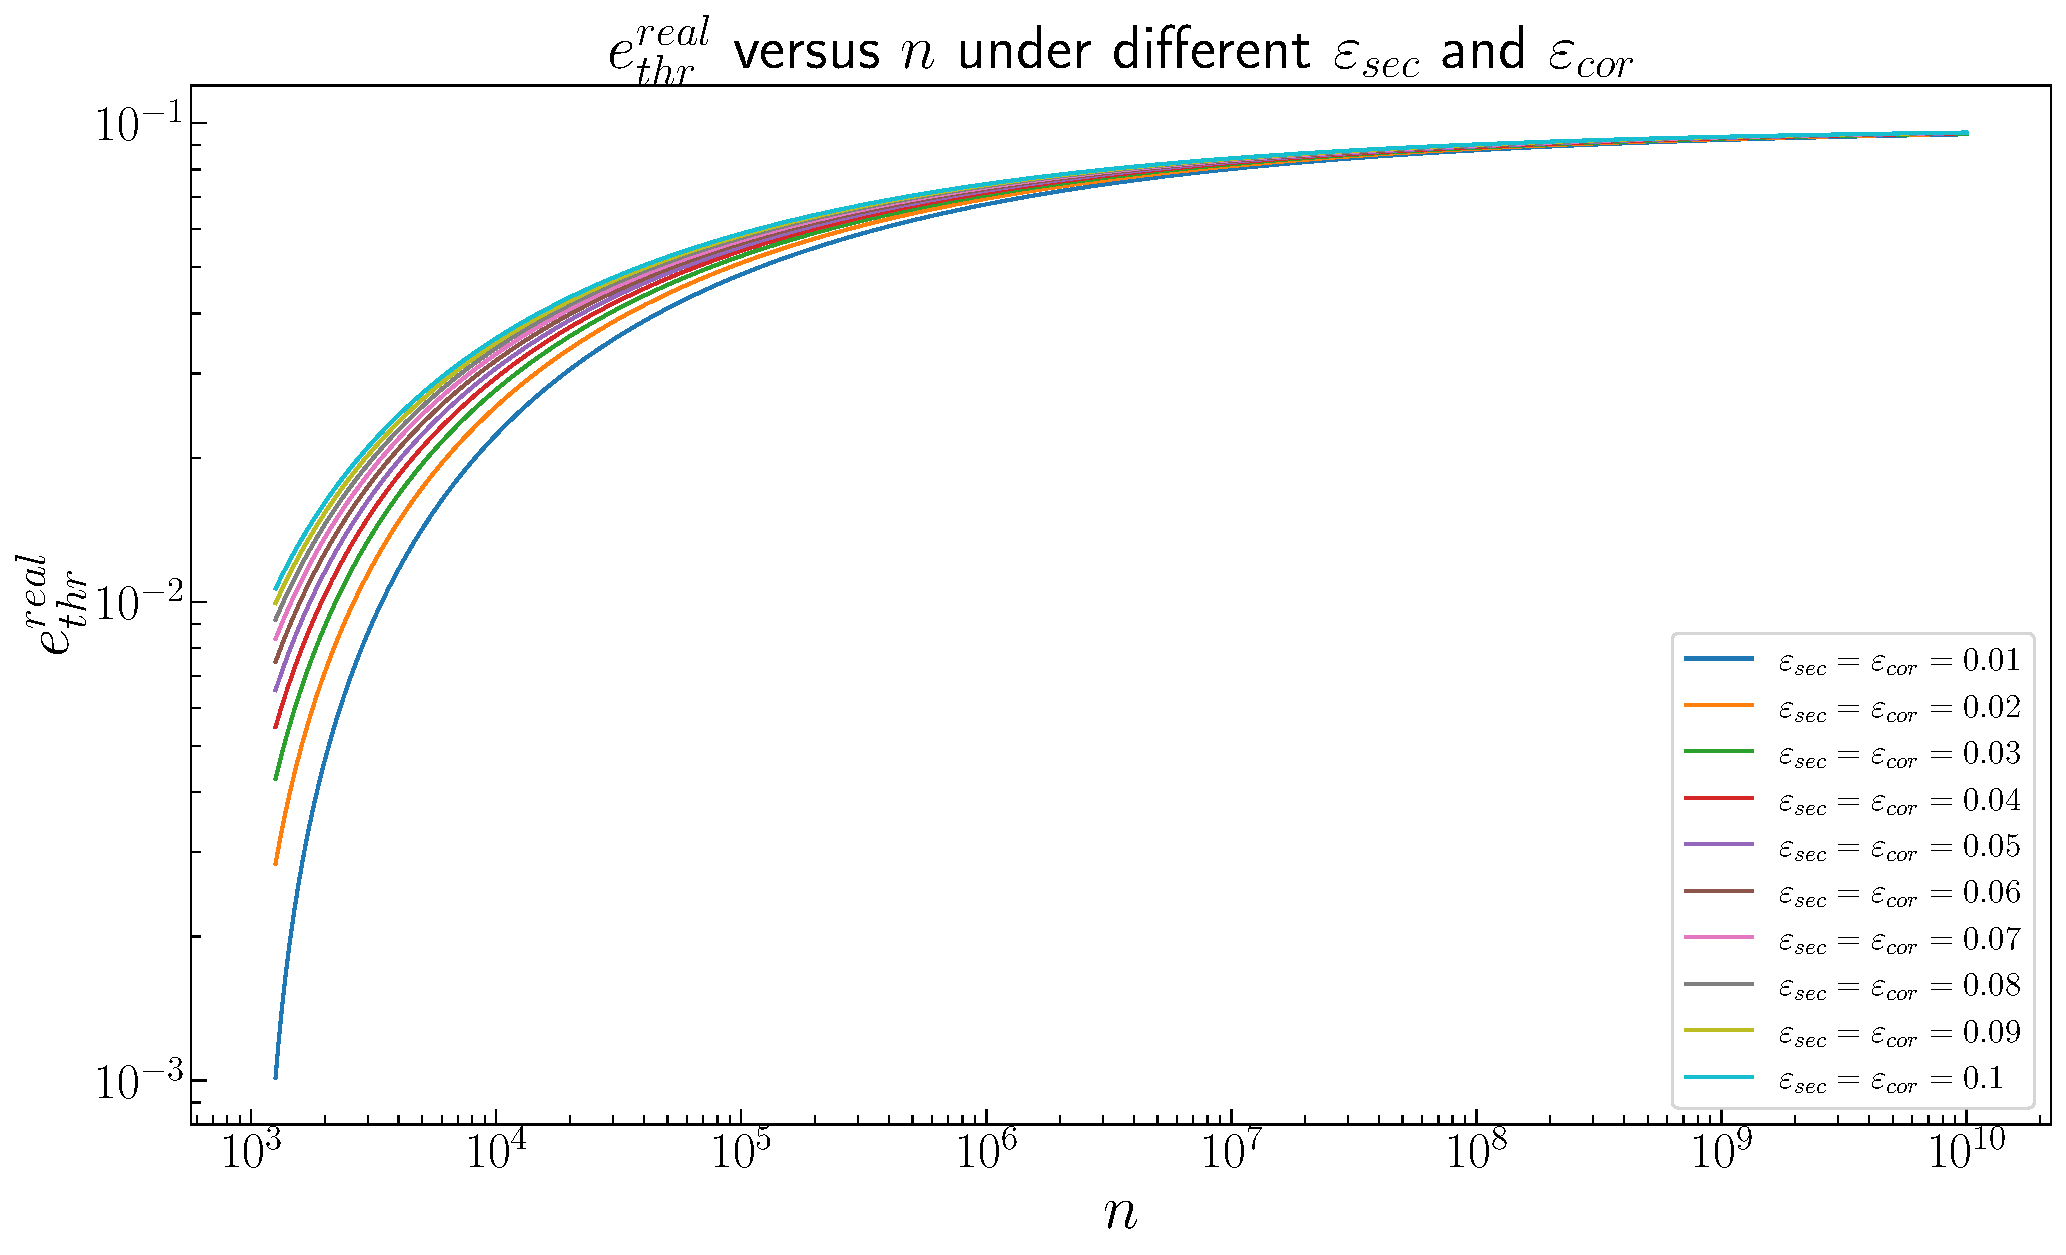
\includegraphics[width=\linewidth]{real_threshold_error_rate.pdf}
    \caption{An estimate on $e_{thr}^{real}$ at different $\epsilon_{sec}$ and $\epsilon_{cor}$ as a function of $n$, we take $k=\sqrt{n}$. Compare this to the theoretical value of $e_{thr}\approx11\%$}
    \label{fig:real_threshold_error_rate}
\end{figure}

Again, even exactly solving this inequality is hard. Thus, to gain an insight into the magnitude of the $e_{thr}^{real}$, we set $\epsilon_{sec}=\epsilon_{cor}=\{0.01, 0.02, 0.03, 0.04, 0.05\}$. The result is shown in Figure~\ref{fig:real_threshold_error_rate}. When $\epsilon_{sec}$ and $\epsilon_{cor}$ are larger, which means we accept a larger failing probability of the protocol or a larger chance that the eavesdropper gains some information, then the realistic threshold key rate $e_{thr}^{real}$ is larger. Also, $e_{thr}^{real}$ becomes larger as $n$ increases, because when $n$ is larger, the results are closer to the asymptotic limits, which is $e_{thr}\approx11\%$.

Then, we will numerically estimate the lower-bound of the overhead $h$ given different channel errors under finite key effect. Recall that in the above sections, we have reviewed the finite-key rate:

\begin{equation}
    r_{real}\approx (q-H_2(e_{tol}+\mu)-1.16H_2(e_{tol}))/c-\frac{\log_2 \frac{2}{\epsilon_{sec}^2\epsilon_{cor}}}{nkc}\\
\end{equation}

\begin{figure}
    \centering
    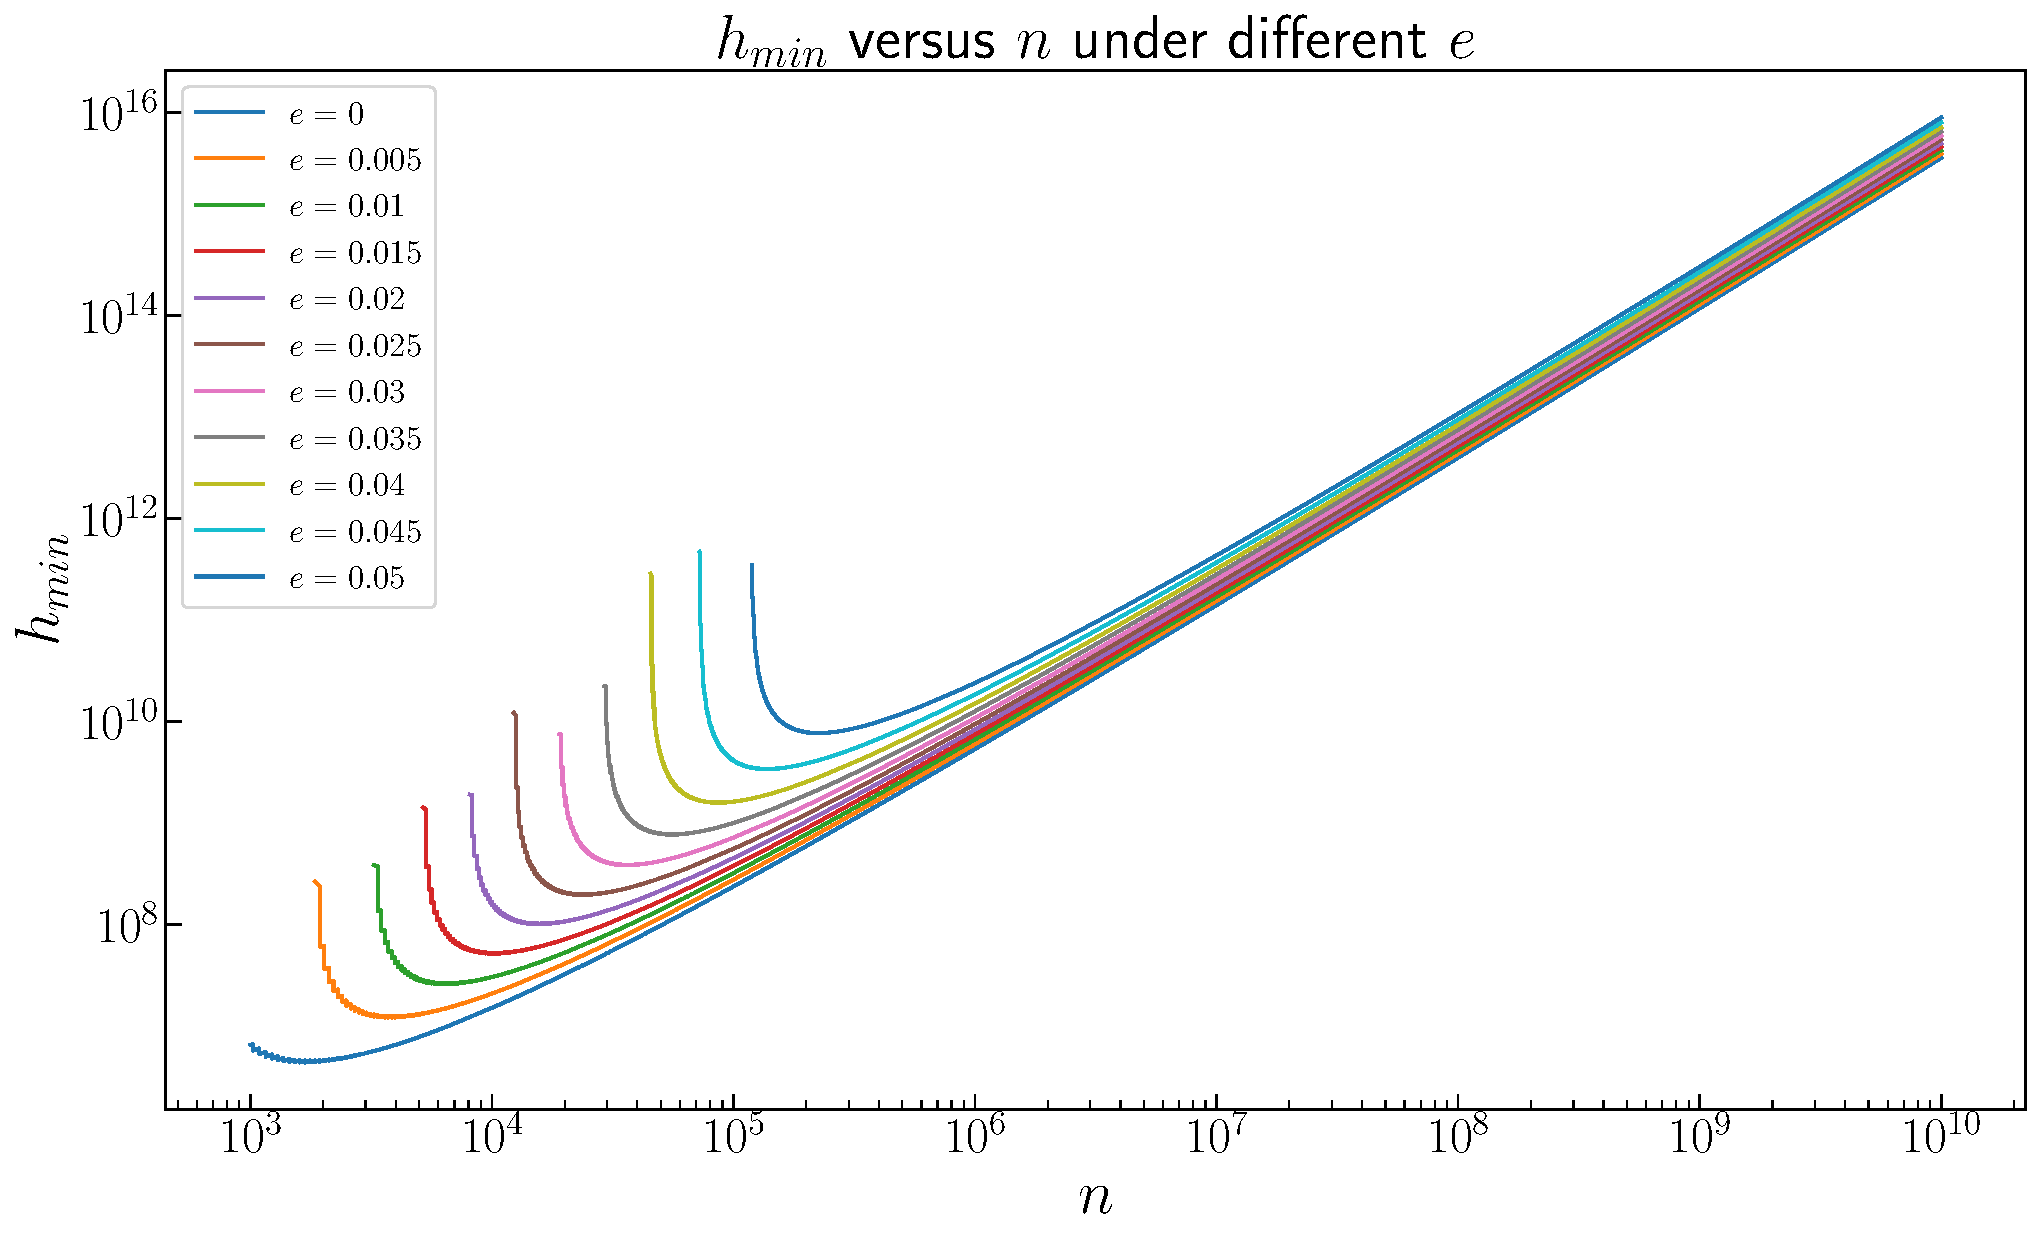
\includegraphics[width=\linewidth]{minimum_overhead_vary_channel_error_rate.pdf}
    \caption{The minimum overhead of $h$, $h_{min}$, as a function of $n$ under different channel error rate $e$, we take $k=\sqrt{n}$ with $b=1/4$, $\epsilon = 0.01$, $\epsilon_{sec}=\epsilon_{cor}=0.01$.}
    \label{fig:minimum_overhead_vary_channel_error_rate}
\end{figure}

\begin{figure}
    \centering
    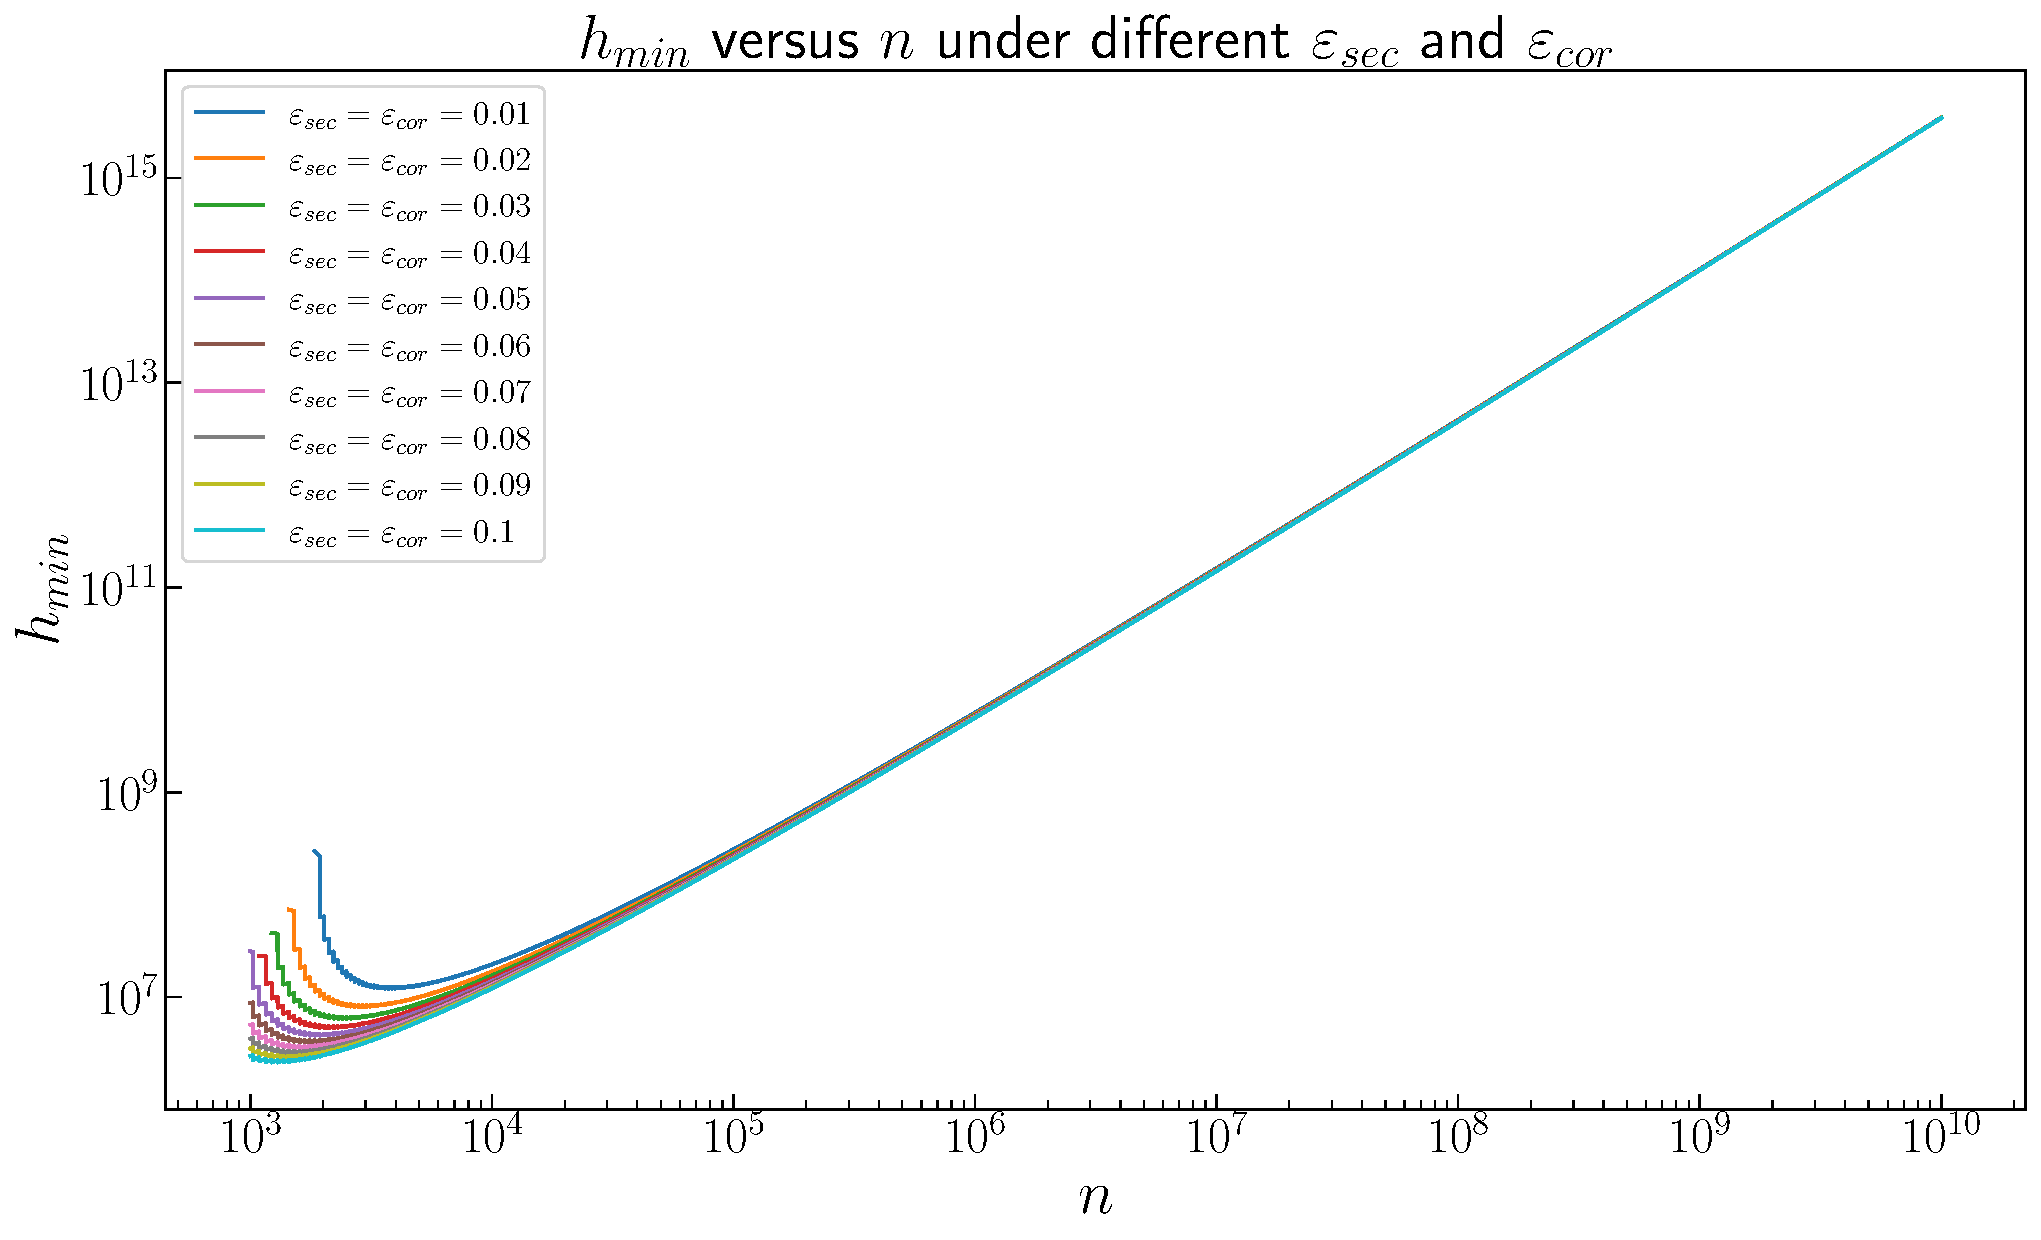
\includegraphics[width=\linewidth]{minimum_overhead_vary_epsilon_cor_sec.pdf}
    \caption{The minimum overhead of $h$, $h_{min}$, as a function of $n$ under different $\epsilon_{cor}$ and $\epsilon_{sec}$, we take $k=\sqrt{n}$ with $b=1/4$, $\epsilon = 0.01$, $e=0.005$.}
    \label{fig:minimum_overhead_vary_epsilon_cor_sec}
\end{figure}

For simulation purposes. To obtain a function of the minimum overhead of $h$, $h_{min}$, as a function of the channel error rate $e$. We assume $c=1.15$, which means about $15\%$ of the qubits are used for error estimation, and in the normal QKD setting, $b=1/4$, take $\epsilon = 0.01$, which is the parameter that governs the probability where Bob obtains more bits than she anticipated, this will be discussed in more detail in section~\ref{sec:Bob_Cheating}, and $\epsilon_{sec}=\epsilon_{cor}=0.01$. The result is shown in Figure~\ref{fig:minimum_overhead_vary_channel_error_rate}. A clear observation is that, the larger the channel error rate, the larger the $h_{min}$, and if the channel error rate is too big, for small $nk$, the finite-key key rate $r_{real}$ is essentially 0, and thus the scheme fails regardless of the overhead resources $h_{min}$.

In Figure~\ref{fig:minimum_overhead_vary_epsilon_cor_sec}, we fixed the channel error rate to be $0.005$, and we plot $h_{min}$ as a function of $\epsilon_{cor}$ and $\epsilon_{sec}$. One can see that only at small $nk$, the value of $\epsilon_{cor}$ and $\epsilon_{sec}$ matters a lot.


\section{Security against Bob}
\label{sec:Bob_Cheating}

In this section, we demonstrate that if Bob follows the protocol in Section~\ref{sec:the_protocol}, then she will gain no extra information on the dataset that Alice holds asymptotically.


\subsection{Bob Gain No Information On Ambiguous Measurement Results}
The first question is whether, for the states that are not unambiguously identified, Bob has any partial knowledge about them? Fortunately, the answer is no; here is the proof. Without loss of generosity, suppose Bob gets a state from Alice, and Bob measures it in $\{\ket{+}, \ket{-}\}$ basis, and obtains the result $\ket{-}$. Then, Alice told Bob that the state prepared is either $\ket{0}$ or $\ket{-}$. With a generalized Positive Operator-Valued Measurement (POVM), the maximum success probability of USD is $1-|\bra{0}\ket{-}|=1-\sqrt{2}/2\approx0.293$, but it requires embedding the qubit into a higher-dimensional Hilbert space using an ancilla or additional modes. For practical considerations, photons have 2 polarizations, so we will start our analysis from the simplest case.


In the simple case, suppose Alice told Bob that the state prepared is either $\ket{0}$ or $\ket{-}$, we can calculate the following probabilities via simple Bayes' theorem 
\begin{equation}
    P(X|Y) = \frac{P(X \cap Y)}{P(Y)}
\end{equation}

Firstly, to illustrate the idea, we restrict ourselves to the strict 2-level case without considering the generalized measurement. For ambiguous cases, we mark Bob as A and Alice as B:
\begin{equation}
    \begin{split}
        P(\text{A gets $\ket{-}$ $|$ B sends $\ket{-}$})&=\frac{0.5\times 0.5}{0.5}=\frac{1}{2}\\
        P(\text{A gets $\ket{0}$ $|$ B sends $\ket{-}$})&=\frac{0.5\times 0.25}{0.5}=\frac{1}{4}\\
        P(\text{A gets $\ket{0}$ $|$ B sends $\ket{0}$})&=\frac{0.5\times 0.5}{0.5}=\frac{1}{2}\\
        P(\text{A gets $\ket{-}$ $|$ D sends $\ket{0}$})&=\frac{0.5\times 0.25}{0.5}=\frac{1}{4}\\
    \end{split}
\end{equation}

Hence, 
\begin{equation}
    \begin{split}
        P(\text{A gets $\ket{-}$ $|$ ambiguous})&=\frac{0.5+0.25}{0.5+0.5+0.25+0.25}=\frac{1}{2}\\
        P(\text{A gets $\ket{0}$ $|$ ambiguous})&=\frac{0.5+0.25}{0.5+0.5+0.25+0.25}=\frac{1}{2}\\
    \end{split}
\end{equation}

Thus, when Bob gets an ambiguous result, she cannot gain any partial information on what Alice prepares. This is intuitively understandable as the 2 results are symmetric. 

\subsubsection{Considering Generalized Measurement}
Now, we will take into account generalized measurement. Suppose Bob can conduct a generalized measurement, which we will show she still gains no partial information from a non-deterministic result.

Without loss of generosity, suppose Alice sends Bob a state, and announces that the state is either $\ket{0}$ or $\ket{-}$, then, Bob can define a generalized POVM elements $Pp, Pq, Pr$, where $Pp+Pq+Pr=I_3$, such that 

\begin{equation}
\begin{split}
    \ket{p}&=\alpha\ket{1}+\beta\ket{2}\\
    \ket{q}&=\gamma\ket{+}+\beta\ket{2}\\
\end{split}
\end{equation}

and $Pp=\ket{p}\bra{p}, Pq=\ket{q}\bra{q}, Pr=I_3-Pp-Pq$. By imposing proper normalization requirements, $\alpha^2+\beta^2=\gamma^2+\beta^2=1$, and orthogonal requirements, $\bra{p}\ket{q}=0$, Simple calculation reveals $\alpha^2=\gamma^2=2-\sqrt{2}, \beta^2=\sqrt{2}-1$. Then, we have

\begin{equation}
    Pp=\left(
\begin{array}{ccc}
 0 & 0 & 0 \\
 0 & \alpha^2 & 0 \\
 0 & 0 & \beta^2 \\
\end{array}
\right), \qquad
Pq=\left(
\begin{array}{ccc}
 \frac{\alpha^2}{2} & \frac{\alpha^2}{2}
   & 0 \\
 \frac{\alpha^2}{2} & \frac{\alpha^2}{2}
   & 0 \\
 0 & 0 & \beta^2 \\
\end{array}
\right),
\end{equation}
\begin{equation}
Pr=\left(
\begin{array}{ccc}
 1-\frac{\alpha^2}{2} &
   -\frac{\alpha^2}{2} & 0 \\
 -\frac{\alpha^2}{2} & 1-\frac{3
   \alpha^2}{2} & 0 \\
 0 & 0 & 1-2 \beta^2 \\
\end{array}
\right)
\end{equation}

To Bob, the state she received is a mixed state,
\begin{equation}
\begin{split}
    \rho_A &= \frac{1}{2}(\ket{0}\bra{0}+\ket{-}\bra{-})\\
    &=\left(
\begin{array}{ccc}
 \frac{3}{4} & -\frac{1}{4} &
   0 \\
 -\frac{1}{4} & \frac{1}{4} &
   0 \\
 0 & 0 & 0 \\
\end{array}
\right)
\end{split}
\end{equation}

If Bob perform the POVM and projected $\rho_A$ into $\ket{p}$, then, Bob can unambiguously conclude that the initial state sent by Alice is $\ket{-}$; similarly, if Bob projected $\rho_A$ into $\ket{q}$, then, Bob can unambiguously conclude that the initial state is $\ket{0}$. Nondeterministic result happened if Bob projected $\rho_A$ into $\ket{r}$, which is the eigenstate of $P_r$.

It is easily checkable that for $\rho_{A0}=\ket{0}\bra{0}$ and $\rho_{A-}=\ket{-}\bra{-}$, the probability of projecting onto $\ket{r}$ is the same, mathematically,

\begin{equation}
    Tr[\rho_{A0}Pr]=Tr[\rho_{A-}Pr]=Tr[\rho_{A}Pr]=\frac{1}{\sqrt{2}}
\end{equation}

Hence, if the non-deterministic result is obtained, Bob cannot gain any partial information on the initial state.



\subsection{Bob Gaining Extra Unintended Information}
Now, the second question is whether Bob can get more than 1 bit of information from Alice's database? Here, we show that the probability of Bob gaining more than 1 bit of data can be made arbitrarily low at the cost of increasing the failure probability of the protocol.

As mentioned before in the Section~\ref{sec:the_protocol}, after Alice and Bob shared imperfect strings $\textbf{x}_N$ and $\textbf{y}_N$ respectively with length $N=kn$, where $n$ is the length of the database held by Alice. Alice will randomly shuffle and reduce it into $n$ blocks, each with $k$ bits. Furthermore, Alice will choose an $[[k, 1, d]]$ QECC and publicly announce it; the chosen QECC is then applied to all $n$ blocks. Eventually, the original length $N=kn$ bit-string is reduced to a bit-string of length $n$, $\textbf{s}_b=\{s_{b0}, s_{b1}, \cdots, s_{bn}\}\in\Sigma^n$ and $\textbf{s}_a=\{s_{a0}, s_{a1}, \cdots, s_{an}\}\in\Sigma^n$ held by Alice and Bob, respectively. 

We claim that the protocol succeeds under the accomplishment of the following criterion: $\exists! i$ where $x_i=y_i$, and for $\textbf{x'}=\{x_0, \cdots, x_{i-1}, x_{i+1}, \cdots, x_n\}$ and $\textbf{y'}=\{y_0, \cdots, y_{i-1}, y_{i+1}, \cdots, y_n\}$, that $I(X', Y')\le \epsilon$ as we described in Section~\ref{sec:formal_definition}. There are three possible failures of the protocol:
\begin{enumerate}
    \item $\nexists i$ such that $x_i=y_i$. Then, Bob cannot obtain any bits.

    \item There exists unique $i_0, \cdots i_l$ and that both $x_{i_v}=y_{i_v}$ for $v=1, \cdots l$. Then, Bob can identify more than 1 bit.

    \item $I(\textbf{x'}, \textbf{y'})>\epsilon$. Then, Bob might be able to identify more than 1 bit.
\end{enumerate}


To avoid the failure of the protocol, Alice needs to choose a QEC code with distance $d\le (1-b)(k-\epsilon)$. Here, we would like to investigate the relationship between $n, k, \epsilon$ and the probability of the protocol failing.

Quantum mechanically, we have shown that for each qubit sent by Alice to Bob, suppose the chance that Bob can unambiguously determine the state without noise is $b$. When the channel error is taken into account, the success probability of unambiguous state discrimination will be lower. However, Bob does not know which of his ``unambiguously determined'' bits are prompted to error; hence, we will treat the error later.

%, suppose the channel error rate is $e$, and we denote $b$ to be the probability that Bob can unambiguously determine the state with channel error. Then,

\textbf{We will show that this protocol is information-theoretically secure against Bob, meaning that with probability $1-p_A$, Bob can gain at most $\epsilon_A$ information, and here, we will find the parameters $\epsilon_A$ in terms of $p_A$.}

Suppose for any $k$ bit string, we can calculate the probability that Alice can unambiguously determine $a$ bits.
\begin{equation}
    p(a) = \binom{k}{a} \left(b\right)^a\left(1-b\right)^{k-a}
\end{equation}

When Alice chooses an $[[k, 1, d]]$ error-correcting code, and set $d \le(1-b)(k-\epsilon)$. Then, for any block of length $k$ bit-string, if Bob can unambiguously determine at least $(b+\epsilon)k$ bits, she can distill $1$ bit from this block of length $k$. Therefore, we now need to compute the probability that Bob can unambiguously determine at least $\left(b+\epsilon\right)k$ bits, this is:
\begin{equation}
\begin{split}
    p(\text{resolving}\ge k(b+\epsilon)) &= \sum_{a\ge k(b+\epsilon)}^k \binom{k}{a}\left(b\right)^a\left(1-b\right)^{k-a}\\
    &=\sum_{a'=0}^{(1-b-\epsilon)k}\binom{k}{k-a'}b^{k-a'}(1-b)^{a'}\\
    &=\sum_{a'=0}^{(1-b-\epsilon)k}\binom{k}{a'}b^{k-a'}(1-b)^{a'}
\end{split}
\end{equation}

Rewriting the dummy index from $a'$ to $a$, we have:
\begin{equation}
    p(\text{resolving}\ge k(b+\epsilon)) = \sum_{a=0}^{(1-b-\epsilon)k}\binom{k}{a}b^{k-a}(1-b)^{a}\equiv p_1
    \label{eq:p_each_block}
\end{equation}


This is the probability for each block that Bob can successfully correct that block and get $1$ bit. The probability of Bob obtaining more than 1 bit is:

\begin{equation}
\begin{split}
    p(A\ gets\ > 1\ bits) &= 1-\left\{[1-p_1]^n+ \binom{n}{1} p_1[1-p_1]^{n-1}\right\}\\ 
    &= 1-\left\{[1-p_1]^n+np_1[1-p_1]^{n-1}\right\}\\
    &=1 + (1 - p_1)^{n-1} (p_1 - n p_1 - 1)
\end{split}
\label{eq:C_cheated}
\end{equation}

Thus, 

\begin{equation}
\begin{split}
    \frac{dp(A\ gets\ > 1\ bits)}{dp_1}&=n(n-1)p(1 - p)^{n-2}\\
    &>0\qquad \text{for $p\in(0, 1)$}
\end{split}
\end{equation}

Simple calculation from equation~\ref{eq:p_each_block} reveals that $p(A\ gets\ > 1\ bits)$ is monotonically increasing with $p_1$ for $p_1\in(0, 1)$. Next, the probability of Bob obtaining no bits, $p_{A, 0}$ is:
\begin{equation}
\begin{split}
    p_{A, 0} =[1-p_1]^n
    \label{eq:C_failed}
\end{split}
\end{equation}

It is trivial that the probability of Bob obtaining no bits is strictly monotonically decreasing with $p_1$.

Both equations~\ref{eq:C_failed} and~\ref{eq:C_cheated} depends on the value of $p_1$. Hence, we will calculate the upper and lower bounds of $p_1$, and give an upper or lower bound of the probabilities of Bob gaining more than 1 bit or no bits at all.

\subsection{Upper bound for Bob gaining more than 1 bit}
\label{sec:Bob_get_more_info}
As in equation~\ref{eq:C_cheated}, the probabilities where Bob gains more than 1 bit $p_{A, >1}$ are monotonically increasing with $p_1$, hence, we can obtain the upper bound of $P(A\ gets\ > 1\ bits)$ by calculating the upper bound of $p_1$.

In equation~\ref{eq:p_each_block}, the probability $p(\text{resolving}\ge k(b+\epsilon))$ is equivalent to the following picture, where we set a binomial random variable $X \sim Bin(k, p)$ for $p=1-b$ and $m = \lfloor pk-\epsilon\rfloor$. 

Then, $p(\text{resolving}\ge k(b+\epsilon))$ can be equivalently transformed to $p(X\le m)$. This is exactly a well-studied problem of the tailed probabilities of a Gaussian distribution. The usual representation of the tailed distribution is:
\begin{equation}
\begin{aligned}
&b_{n, k}(p):=\binom{n}{k} p^k (1-p)^{n-k}\\
&B_{n, k}(p):=\sum_{j=0}^k b_{n, j}(p)=\sum_{j=0}^k\binom{n}{j} p^j (1-p)^{n-j}
\end{aligned}
\end{equation}

One of the most popular upper bounds for $B_{n,k}(p)$ is the Chernoff bound
\begin{equation}
    B_{n,k}(p)\le e^{-nD\left(\frac{k}{n}\|p\right)}
    \label{eq:Chernoff_bound}
\end{equation}

which characterizes the exponential decay rate of the tail probability, where $D(p||q)$ represents the Kullback-Leibler (K-L) divergence, 
\begin{equation}
D(f \| p):=f \ln \frac{f}{p}+(1-f) \ln \frac{1-f}{1-p}
\end{equation}

Using this result, the $p(\text{resolving}\ge k(b+\epsilon)) = p(X\le m) = B_{k, (1-b-\epsilon)k}(1-b)$, using equation~\ref{eq:Chernoff_bound},
\begin{equation}
    B_{k, (1-b-\epsilon)k}(1-b)\le e^{-kD\left(1-b-\epsilon\|1-b\right)}
\end{equation}

Since, $\epsilon\ll1$, we would like to approximate the K-L divergence $D(1-b-\epsilon\|1-b)$

\begin{equation}
\begin{split}
    &D(1-b-\epsilon\|1-b)\\&=(1-b-\epsilon)\ln\left(\frac{1-b-\epsilon}{1-b}\right)+(b+\epsilon)\ln\left(\frac{b+\epsilon}{b}\right)\\
    &\approx \frac{\epsilon^2}{2b(1-b)}+O(\epsilon^3)
    \end{split}
\end{equation}

Hence, 
\begin{equation}
\begin{split}
p_1=B_{k, (1-b-\epsilon)k}(1-b)&\le e^{-kD\left(1-b-\epsilon\|1-b\right)}\\
%not sure if this is correct!!!!!!!!!!!!!!!!!!!!!!!!!!
&\le e^{-\frac{k\epsilon^2}{2b(1-b)}}\\
%&\le 1-\frac{k\epsilon^2}{2b(1-b)}
\end{split}
\end{equation}

For simplicity, write $c=\frac{k}{2b(1-b)}$, then,

\begin{equation}
    p_1\le  e^{-c\epsilon^2}
\end{equation}

Substitute this result back into equation~\ref{eq:C_cheated}, and we denote the probability where Bob gets more than 1 bit to be $p_{A, >1}$. We get:
\begin{equation}
    \begin{split}
        p_{A, >1} &=1-\left[(1-p_1)^n+np_1(1-p_1)^{n-1}\right]\\
        &\le 1-\left[(1-e^{-c\epsilon^2})^n+n(e^{-c\epsilon^2})(1-e^{-c\epsilon^2})^{n-1}\right]\\
        &=1-(1-e^{-c\epsilon^2})^{n-1}\left[1+(n-1)e^{-c\epsilon^2}\right]
        %&=1-c^n\epsilon^{2n}-nc^{n-1}\epsilon^{2n-2}+nc^n\epsilon^{2n}\\
        %&=1-c^{n-1}\epsilon^{2n-2}\left[n+(1-n)c\epsilon^2\right]\\
        %&\le 1-nc^{n-1}\epsilon^{2n-2}\left[1-c\epsilon^2\right]\\
        %&=1-O\left[nk^{n-1}\epsilon^{2n-2}(1-k\epsilon^2)\right]
        %&=1+(n-1)c^n\epsilon^{2n}-nc^{n-1}\epsilon^{2n-2}\\
        %&= 1+nc^n\epsilon^{2n}-nc^{n-1}\epsilon^{2n-2}\\
        %&=1-nc^{n-1}\epsilon^{2n-2}\left(1-c\epsilon^{2}\right)\\
    \end{split}
    \label{eq:upper_bound_C_cheated}
\end{equation}

Let us denote $p_{A,i}$ as the probability that Bob can resolve $\ge k(b+\epsilon)$ bits in $i$ blocks. Therefore, trivially $\sum_{i=0}^n P_{A, i}=1$, and 
\begin{equation}
    p_{A, i} = \binom{n}{i}p_1^i(1-p_1)^{n-i}
\end{equation}
The average number of bits obtained by Bob $Q_{A}$ is given by
\begin{equation}
\begin{split}
    Q_{A} &= \sum_{i=0}^n ip_{A, i}\\
    &=\sum_{i=0}^ni\binom{n}{i}p_1^i(1-p_1)^{n-i}
\end{split}
\end{equation}

Denotes $Q_{A, \ge i}$ to be the average number of bits obtained by Bob consider only the tailed distribution $p_{A, \ge i}$
\begin{equation}
    \begin{split}
    Q_{A, \ge2}
    &= \sum_{i=2}^n ip_{A, i}\\
    &=\sum_{i=2}^ni\binom{n}{i}p_1^i(1-p_1)^{n-i}\\
    &=np_1-np_1(1-p_1)^{n-1}\\
    &=np_1(1-(1-p_1)^{n-1})\\
    &\le np_1(n-1)p_1\\
    &=n(n-1)p_1^2\\
    %&=n(n-1)(1-c\epsilon^2)^2
    \end{split}
\end{equation}
Hence, the average number of bits Bob gets, provided that Bob gains more than 1 bit, is:
\begin{equation}
    \epsilon_A = n(n-1)(1-c\epsilon^2)^2
\end{equation}

Hence, with probability $1- p_{A, \ge 1}$, Bob will gain less than $\epsilon_A=n(n-1)(1-c\epsilon^2)^2$ bits of unintended information.

Hence, given a tolerable probability $p$, we can find a value of $k$ and $\epsilon$ such that the probability of Bob gaining more than 1 bit is arbitrarily small. It is quite clear that equation~\ref{eq:upper_bound_C_cheated} shows the upper bound of the probability of Bob gaining more than 1 bit increase with $\epsilon$. Which means, our scheme is information-theoretically secure against Bob gaining extra information.

Unfortunately, the probability of Bob gaining more than 1 bit also grows with $\epsilon$, as in equation~\ref{eq:C_failed}. Therefore, there is a fundamental trade-off between the probability of Bob getting more than 1 bit and the probability of Bob getting no bits at all.

Notice that in this section, where we discussed the probability of Bob obtaining extra information, we made no assumptions on the asymptotic limits of the channel key rates, and the bounds presented in that section should be tight even if we consider the realistic codes and finite-key.

\subsection{Bob Gains no Information from the blocks that are not correctable}

As we presented in Section~\ref{sec:Bob_Cheating}, the protocol's success depends on the criteria. In the above subsections, we have given bounds to the probability of that with the $[[k, 1, d]]$ QEC code, Bob can correct more than 1 block, or Bob can correct no blocks. In this subsection, we target the third failing possibility: whether, for the uncorrectable blocks, Bob can obtain any useful partial information. The theorems in QEC code guarantee that with the uncorrectable blocks, with large probability, Bob gains negligible information; this is a well-known result, we quote the theorem of QEC here.

This means that for a block of $k$ bits, which is not correctable by Bob, Bob gains asymptotically no information at all. Hence, when Bob tries to use the $[[k, 1, d]]$ code to apply to the uncorrectable blocks, the result is random. Mathematically, if we denote the QEC code as $Q$, and block $i$ is the only block that Bob can correct. Then for the 2 shifted keys except at location $i$,

\begin{equation}
    \mathbf{x'}=[Q(\mathbf{s_{b1}}), \cdots Q(\mathbf{s_{bi-1}}), Q(\mathbf{s_{bi+1}}), \cdots, Q(\mathbf{s_{bn}}) ])
\end{equation}

\begin{equation}
    \mathbf{y'}=[Q(\mathbf{s_{c1}}), \cdots Q(\mathbf{s_{ci-1}}), Q(\mathbf{s_{ci+1}}), \cdots, Q(\mathbf{s_{cn}}) ])
\end{equation}

will obey that,

\begin{equation}
    I(\mathbf{x'}, \mathbf{y'})<\epsilon
\end{equation}

Then, Bob gains asymptotically no information from the uncorrectable blocks.


\section{Security Against Alice}

In our assumption, the quantum channel is completely controlled by Eve, where neither Bob nor Alice has control over the quantum channel.

Alice may cheat by trying to gain information on the bits that Bob is interested in. Therefore, any cheating strategy during the initial QKD phase, corresponding to steps 1 and 2 in the above protocol, will have the potential hazard of leaking information to Eve. Bob only communicates with Alice twice, once during the initial error estimation, whereby we assume that the communication channel is completely controlled by Eve. In fact, Bob may be able to gain some advantages by exaggerating the channel error rate, which will be later discussed in Section~\ref{sec:Bob_cheating_error_rate}. 

Also, note that moving from qubits to qudits does not give Alice any fundamental cryptographic advantage over Bob; it does not evade the usual no‑go theorems for mistrustful two‑party cryptography~\cite{Multiphoton_side_channel_attack1, Multiphoton_side_channel_attack2}. The only ``advantage'' he gains by secretly using a higher‑dimensional space in a nominally 2D protocol is the ability to mount side-channel-type attacks that exploit Bob’s implementation assumptions, which is precisely viewed as breaking the protocol, as we assumed that Alice is not colluding with Eve, rather than improving it.

For example, when our implementation assumes a 2-level qubit (e.g., single‑photon polarization) but a malicious Alice actually uses multi‑photon pulses or extra degrees of freedom (time, frequency, spatial mode, etc.)~\cite{Multiphoton_side_channel_attack1}. In that case, he can sometimes correlate which pulses click which of Bob’s threshold detectors, to gain nontrivial information about Bob’s measurement choices or outputs~\cite{Multiphoton_side_channel_attack1}. However, this kind of attack is mainly related to experimental apparatus and should be classified as side-channel attacks, which are outside the scope of this paper.

Also, Alice will not gain any advantage in marking up the channel error rate as long as the channel error rate is symmetric between the bit-flip and phase-flip error; however, Alice does gain an advantage if the error rate is asymmetric between bit-flip and phase-flip, which is discussed later in Section~\ref{sec:Alice_cheating_asymmetric_measurement}.

However, will Alice gain any unfair advantage if he lies (i.e., he does not prepare the states in $\{\ket{0}, \ket{1}, \ket{+}, \ket{-}\}$, but some other single-qubit or entangled states)?

The answer is no, as the no-communication (no-signaling) theorem states that for any bipartite state, local operations or measurements (including randomized basis choices) on one subsystem cannot influence the marginal statistics or state accessible to the distant subsystem, thereby forbidding information transfer without classical communication~\cite{No_signaling1, No_signaling2}. Which means Alice cannot gain any information on Bob's basis choice and measurement results. Thus, after the channel error estimation stage is over, Alice cannot gain any information on the measurement basis and results of the other states that Bob does not reveal. Hence, Alice will not gain any unfair advantages if he prepares other quantum states or even entangled states. However, using some erroneous states can be beneficial to avoid Bob cheating, and we present the detailed analysis in Section~\ref{sec:Bob_cheating_error_rate}.

The last time Bob communicates with Alice is when Bob returns the permuted index strings. As a theoretical analysis, we assume the measurement performed by Bob is symmetric, meaning that the error rate of the measurements in the H-V basis and the D-A basis is the same, in fact, if the measurement error rate of H-V basis and the D-A basis is not the same, it will potentially leak information to Alice, as we will show in Section~\ref{sec:potential_cheating}.

Also, each detection event is independent, so Alice has no way to know which set of qubits is unambiguously determined by Bob. Hence, Bob returns the permuted blocks in step 9 of the protocol~\ref{sec:the_protocol} will look no different from a random string to Alice.

\section{Decoy State QKD Setting}
In most realistic experimental QKD settings, to avoid the photon-number-splitting (PNS) attacks, one always needs to use decoy-state QKD. We would like to show that our scheme works perfectly well with the decoy-state setting. In this section, without loss of generality, we demonstrate the key idea using a specific BB84 QKD protocol where the raw key is generated by the $X$ measurement results, and channel phase error checks are done by the $Z$ measurement results. Other BB84 QKD schemes can be easily generalized.

\section{Review of Decoy-State QKD}
\label{sec:review_decoy_state_qkd}

Practical implementations of QKD often rely on highly attenuated coherent laser pulses, which follow a Poisson photon-number distribution. This introduces the risk of the PNS attack, where an eavesdropper can selectively block single-photon pulses and split multi-photon pulses, retaining one photon while forwarding the rest to Alice, thus gaining information without being detected.

To counter the PNS attack and achieve secure key rates comparable to those of true single-photon sources, the decoy-state method was introduced. In this approach, Bob randomly varies the intensity of her emitted laser pulses, preparing them in either signal states or one or more decoy states. Eve, unable to determine the intensity class of a given pulse beforehand, must apply the same interaction to all pulses containing the same number of photons.

By analyzing the transmission statistics (yields and error rates) associated with the different intensity settings, Alice and Bob can accurately estimate the crucial parameters needed for security proofs: the yield and the quantum bit error rate (QBER), specifically for the single-photon pulses. Suppose Alice and Bob uses use $k\ge2$ different photon intensities labeled $\mu_1, \mu_2, \cdots, \mu_k \ge 0$, each with probability $p_{\mu_1}, p_{\mu_2}, \cdots, p_{\mu_k}$. The observed average yield per photon pulse is

\begin{equation}
    Q_{A, \mu_n} = \sum_{m=0}^{+\infty}\frac{\mu_n^mY_{A, m}\exp{(-\mu_n)}}{m!}
\end{equation}

Here, $Y_{A, m}$ represents the probability of Bob detecting at least one photon if there are $m$ photons in the original pulse. In general, Bob can choose to measure in either the $X$ or $Z$ basis, so $A=X$ or $Z$. Similarly, the observed average bit error rate $E_{A,\mu_n}$ is given by

\begin{equation}
    Q_{A, \mu_n} E_{A, \mu_n} = \sum_{m=0}^{+\infty}\frac{\mu_n^mY_{A, m}e_{A, m}\exp{(-\mu_n)}}{m!}
\end{equation}
Here, $e_{A, m}$ represents the bit error rate if there are $m$ photons in the original pulse prepared in the $A$ basis.

Infinitely many intensities $\mu_n$ are needed to determine all the $Y_{A, m}$’s and $e_{A, m}$’s assuming the functions are well-behaved, fortunately, to get a lower bound of the one-way private key rate $r_{decoy}$, we only require lower bounds on $Y_{X, 0}$, $Y_{X, 0}$; as well as an upper bound on $H_2(e_{Z, 1})$. Because $r_{decoy}$ is defined as the number of final secure private key length divided by the expected number of photon pulses sent through the channel.

\begin{equation}
    \begin{aligned}
&R_{decoy}=\\
&p_{\mathrm{X}}^2\left\{\langle\exp (-\mu)\rangle Y_{\mathrm{X}, 0}+\langle\mu \exp (-\mu)\rangle Y_{\mathrm{X}, 1}\left[1-H_2\left(e_p\right)\right]\right. \\
& \left.-\left\langle Q_{\mathrm{X}, \mu} H_2\left(E_{\mathrm{X}, \mu}\right)\right\rangle-\frac{\left\langle Q_{\mathrm{X}, \mu}\right\rangle}{\ell_{\mathrm{raw}}}\left[6 \log _2 \frac{\chi(k)}{\epsilon_{\mathrm{sec}}}+\log _2 \frac{2}{\epsilon_{\mathrm{cor}}}\right]\right\} .
\end{aligned}
\end{equation}

Where $p_X$ is the probability of Alice and Bob preparing or measuring in the $X$ basis. And the symbol $\langle f(\mu)\rangle = \sum_{n=1}^k p_{\mu_n} f(\mu_n)$, and $H_2(x)=-x\log_2x-(1-x)\log_2(1-x)$ is the binary entropy function. $\chi(k)$ is a QKD scheme-specific factor depending on the number of photon intensities $k$ as well as the detailed security analysis used, and $\chi(3)=21$.

It has been previously studied by H.F. Chau in Ref.~\cite{Decoy_state_key_rate1} that, using $k$ different intensities,
\begin{equation}
    Y_{B, 0} \geqslant \max \left(0, \sum_{i=k_0}^k \frac{-Q_{\mathrm{B}, \mu_i}^{\left\langle\left\langle k_0-i\right\rangle\right\rangle} \exp \left[\mu_i\right] \hat{\prod}_{j \neq i} \mu_j}{\hat{\prod}_{t \neq i}\left[\mu_i-\mu_t\right]}\right)
    \label{eq:YB0_general}
\end{equation}
\begin{equation}
    Y_{B, 1} \geqslant \max \left(0, \sum_{i=3-k_0}^k \frac{-Q_{\mathrm{B}, \mu_i}^{\left\langle\left\langle k_0-i\right\rangle\right\rangle} \exp \left[\mu_i\right] \hat{S}_i}{\hat{\prod}_{t \neq i}\left[\mu_i-\mu_t\right]}\right)
    \label{eq:YB1_general}
\end{equation}
and
\begin{equation}
    Y_{\mathrm{Z}, 1} e_{\mathrm{Z}, 1} \leqslant \min \left(\frac{1}{2}, \sum_{i=k_0}^k \frac{\left[Q_{\mathrm{Z}, \mu_i} E_{\mathrm{Z}, \mu_i}\right]^{\left\langle\left\langle k_0-i\right\rangle\right\rangle} \exp \left[\mu_i\right] \hat{S}_i}{\hat{\prod}_{t \neq i}\left[\mu_i-\mu_t\right]}\right)
    \label{eq:YZ1eZ1_general}
\end{equation}

And, according to Ref.~\cite{Decoy_state_key_rate1}, using four to five photon intensities will likely give optimal key rates using realistic parameters. However, most experimental setups use 3 intensities $\mu_1>\mu_2>\mu_3\ge 0$, where $\mu_1\gtrsim0.5$, $0.01\lesssim\mu_2\lesssim0.1$ and $\mu_3\approx0$, and equations ~\ref{eq:YB0_general},~\ref{eq:YB1_general}, ~\ref{eq:YZ1eZ1_general} can be reduced to the normally used formula,

\begin{equation}
    Y_{\mathrm{B}, 0} \geqslant \frac{\mu_2 Q_{\mathrm{B}, \mu_3}^{\langle 1\rangle} \exp \left(\mu_3\right)-\mu_3 Q_{\mathrm{B}, \mu_2}^{\langle\langle 0\rangle\rangle} \exp \left(\mu_2\right)}{\mu_2-\mu_3}
\end{equation}

\begin{equation}
    \begin{aligned}
& Y_{\mathrm{B}, 1} e_{\mathrm{B}, 1} \\
& \quad \leqslant \frac{\left(Q_{\mathrm{B}, \mu_2} E_{\mathrm{B}, \mu_2}\right)^{\langle\langle 0\rangle\rangle} \exp \left(\mu_2\right)-\left(Q_{\mathrm{B}, \mu_3} E_{\mathrm{B}, \mu_3}\right)^{\langle\langle 1\rangle\rangle} \exp \left(\mu_3\right)}{\mu_2-\mu_3}
\end{aligned}
\end{equation}
and
\begin{equation}
    \begin{array}{r}
Y_{\mathrm{B}, 1} \geqslant \frac{\mu_1}{\mu_1\left(\mu_2-\mu_3\right)-\mu_2^2+\mu_3^2}\left\{Q_{\mathrm{B}, \mu_2}^{\langle\langle 1\rangle\rangle} \exp \left(\mu_2\right)-Q_{\mathrm{B}, \mu_3}^{\langle\langle 0\rangle\rangle}\right. \\
\left.\quad \times \exp \left(\mu_3\right)+\frac{\left(\mu_2^2-\mu_3^2\right)\left[Y_{\mathrm{B}, 0}-Q_{\mathrm{B}, \mu_1}^{\langle\langle 0\rangle\rangle} \exp \left(\mu_1\right)\right]}{\mu_1^2}\right\}
\end{array}
\end{equation}

Provided that $\mu_1>\mu_2+\mu_3$. In the above equations, $Q_{\mathrm{B}, \mu_2}^{\langle\langle 1\rangle\rangle}$ means  $Q_{\mathrm{B}, \mu_2}+(-1)^i\Delta Q_{\mathrm{B}, \mu_2}$, where the $\Delta$-ed quantities represent the upper bounds on the statistical fluctuation. Using the Hoeffding inequality, these fluctuations can be taken to be at most

\begin{equation}
    \Delta Q_{\mathrm{B}, \mu_n}=\frac{\left\langle Q_{\mathrm{B}, \mu}\right\rangle}{p_{\mu_n}}\left\{\frac{\ln \left[\frac{\chi(k)}{\epsilon_{\mathrm{sec}}}\right]}{2 s_{\mathrm{B}}}\right\}^{1 / 2}
\end{equation}
and
\begin{equation}
    \Delta\left(Q_{\mathrm{Z}, \mu_n} E_{\mathrm{Z}, \mu_n}\right)=\frac{1}{p_{\mu_n}}\left\{\frac{\left\langle Q_{\mathrm{Z}, \mu}\right\rangle\left\langle Q_{\mathrm{Z}, \mu} E_{\mathrm{Z}, \mu}\right\rangle \ln \left[\frac{\chi(k)}{\epsilon_{\mathrm{sec}}}\right]}{2 s_{\mathrm{Z}}}\right\}^{1 / 2}
\end{equation}
Here, $s_A$ is the number of bits that Alice prepares, and Bob successfully measures in the $A$ basis. Trivially, $s_X=l_{raw}$ and $s_Z\approx(1-p_X)^2s_X/p_X^2$.

And, due to the finite key length effect, the phase error rate of the single-photon events in the raw key is upper bounded by
\begin{equation}
    \begin{aligned}
e_p \leqslant & e_{\mathrm{Z}, 1}+\bar{\gamma}\left(\epsilon_{\mathrm{sec}} / \chi(k), e_{\mathrm{Z}, 1}, s_{\mathrm{Z}} Y_{\mathrm{Z}, 1}\langle\mu \exp (-\mu)\rangle /\left\langle Q_{\mathrm{Z}, \mu}\right\rangle\right. \\
& \left.s_{\mathrm{X}} Y_{\mathrm{X}, 1}\langle\mu \exp (-\mu)\rangle /\left\langle Q_{\mathrm{X}, \mu}\right\rangle\right)
\end{aligned}
\end{equation}

with probability at least $1 - \epsilon_{sec}/χ (k)$, where
\begin{equation}
    \bar{\gamma}(a,b,c,d) \equiv \sqrt{\frac{(c+d)(1-b)b}{cd}} \ln \left[ \frac{c+d}{2\pi cd(1-b)ba^{2}} \right]
\end{equation}

\subsection{Decoy-State QKD for SPIR}

As we have proven in the section~\ref{sec:QECC_existence}, all we required is that the error rate $e'$ of each block 
\begin{equation}
    e'=\frac{(1-b-\epsilon)k}{(k+hr/n)(1+e)}
\end{equation}
is smaller than the threshold error rate $e_{thr}$, then, there exists a SPIR scheme that has a greater-than-0 rate.

Here, we assume $\mu_1 = 0.5, \mu_2 = 0.1$ and $\mu_3=0$.



\section{Potential Cheating Methods}
\label{sec:potential_cheating}

In this section, we will briefly discuss some possibilities of either party cheating in the protocol.

\subsection{Alice's Cheating Strategy for Bob's Asymmetric Measurement}
\label{sec:Alice_cheating_asymmetric_measurement}

Here, we would like to investigate the case that, suppose in Bob's lab, the measurement is asymmetric, hence, the probability of unambiguous state discrimination is also asymmetric. Suppose, when Alice sends a state prepared in $\{\ket{0}, \ket{1}\}$ basis, USD succeeds with probability $p_1$, and Alice sends a state prepared in $\{\ket{+}, \ket{-}\}$ USD succeeds with probability $p_2$, and $p_1\ne p_2$. Without loss of generality, let us assume $p_1> p_2$. This is a realistic asymmetric error model, because the asymmetric error in different bases can be due to the quantum communication cable or the measurement device itself, which may affect the success probability of USD in different bases. Denote the overall probability of unambiguously determining a state to be $p=(p_1+p_2)/2$

Alice might be able to cheat by shuffling the blocks differently. Alice may cheat as follows: in each block, Alice will put an asymmetric number of qubits in the $\{\ket{0}, \ket{1}\}$ and $\{\ket{+}, \ket{-}\}$ bases. When Bob chooses the measurement basis at random, as we argued before, if Alice prepares the qubit in one basis, USD is possible only when Bob measures in the complementary basis.

Then, for a specific block of length $k$, suppose Alice put $m$ qubits in $\{\ket{0}, \ket{1}\}$ basis and $(k-m)$ qubits in $\{\ket{+}, \ket{-}\}$ basis, then the mean number of qubits that can be unambiguously determined is $mp_1+(k-m)p_2$, this number range from $kp_2$ to $kp_1$. Which means, if there is a block with all qubits prepared in $\{\ket{0}, \ket{1}\}$ basis, while the other blocks have half qubits in each basis, then, there is a much higher likelihood that Bob will only be able to determine the bit from that particular block. Alice can see where Bob arranged that block to get an idea of which bit Bob is interested in.

There are multiple solutions: If Bob knows that her measurement is asymmetric, she can artificially add some noise sampled from a random number generator to make the measurement result look symmetric. 

Another better way (which may cause a larger overhead) is to modify the steps of the protocol slightly. That, instead of asking Alice to shuffle and arrange the qubits into $n$ blocks randomly, we can let Bob do it. However, she must do it before Alice reveals partial information about the state; otherwise, there is a trivial way for Bob to cheat. This method should be secure, but if Bob eventually finds out that she cannot correct any blocks, Alice and Bob have to abort the protocol and start everything again, which may cause a large overhead.

\subsection{Bob's Cheating Strategy by Exaggerating the channel error Rate}
\label{sec:Bob_cheating_error_rate}

Bob can cheat by exaggerating the channel error rate and fooling Alice into choosing a suboptimal QEC code, thereby cheating.

During step 2 in~\ref{sec:the_protocol}, if Bob deliberately lies to Alice by adding some classical noise during the error rate estimation, she can artificially boost the error rate to be higher. For example, suppose the real quantum channel error rate is $p_r$ and Bob is dishonest about the measurement results, and makes the error rate of the channel look like $p_f$. Then Alice will be tricked into choosing a more powerful QECC that corrects more errors, which then means Bob has a higher chance of decoding each block on which they operate the QECC.

Unfortunately, it is impossible to catch Bob cheating over a general quantum channel described by a completely positive trace-preserving (CPTP) map, because unconditional strong lie detection is impossible in the BB84 setting. The reason behind is that Bob faking several measurement results by classical uncertainty is equivalent to some noise happening in the channel, and Bob somehow gains information about the noise.

Bob can do the following, since Alice would like to get an accurate estimate of $p_r$ from the error estimation process with Bob, where Bob tried to exaggerate it to $p_f$. However, Bob wants the whole protocol to work, so Bob would like to keep $p_f<e_{thr}$, where $e_{thr}$ is the threshold error rate discussed in Section~\ref{sec:QECC_existence}. In the original protocol, since Alice and Bob both publicly announce basis and measurement results, suppose they publicly announce it one by one. Then, suppose Alice is honest, Bob can know an estimate of the actual error rate $p_r$, and if $p_r<e_{thr}$, Bob can artificially add some noise to her measurement result by randomly flipping the measurement result with a small probability to make $p_f\approx_{e_{thr}}$ and gain unfair advantage.

Therefore, there is a natural trade-off between the success probability of the protocol and the chance that Bob will gain more information than she requested. Although in general, catching Bob cheating by exaggerating the channel error rate is impossible, there are ways to reduce the willingness of Bob to exaggerate the channel error rate by scaring Bob that the protocol may fail. One of the possible ways to do it is for Alice to artificially add some noise to several qubits when he sends the qubits to Bob.

We modify the first few steps of the protocol in Section~\ref{sec:the_protocol} as follows: 
\begin{enumerate}
    \item When Alice sends the states to Bob, he will also send some erroneous states $\ket{0'}, \ket{1'}, \ket{+'}, \ket{-'} $ in between the normal states $\ket{0}, \ket{1}, \ket{+}, \ket{-}$, he sends the erroneous states in between normal states, so that Bob does not know which states are normal and which states are erroneous.
    
    \item \textbf{Channel error estimation stage}: Since Bob does not know which states are normal or erroneous. Alice will first randomly choose several states to publicly announce the preparation basis, and the state prepared, even if the states are erroneous $\ket{x'}, x\in\{0, 1, +, -\}$.

    \item Bob will also publicly announce the measurement basis and result of the selected states, and they will estimate the channel error rate in the presence of erroneous states.

    \item Bob does not know how many states are erroneous states, so if she decides to cheat by exaggerating the channel error rate, she might risk the whole protocol failing. Thus, she has less willingness to exaggerate the channel error rate.

    \item Alice knows which states are erroneous, so he can estimate the actual channel error rate by discarding the erroneous states selected, and check if this actual channel error rate is tolerable.

    \item If the actual error rate is tolerable, Alice will announce which states are erroneous and discard those states, then they proceed with the protocol as stated in Section~\ref{sec:the_protocol} with the actual channel error rate.
\end{enumerate}

In this modified protocol, Alice will choose some of the states and send the erroneous states, so when Alice selects the states for error estimation, Alice can make the error an arbitrary number $p_b>p_r$ or even $p_b>e_{thr}$. Then, Bob does not know how many states prepared by Alice are erroneous. Suppose Bob's priority is to make the whole protocol work, then she needs to be quite honest about the measurement basis and the results she obtained. 

At the end, through the use of erroneous states, Alice and Bob will have a shared error rate estimate $p_b$, and Alice will have a private error rate estimate of $p_r'$, obtained by not considering all erroneous states. If $p_r'<e_{thr}$, then Alice will announce that the real error rate passed, and publicly announce $p_r$ and the erroneous states if there are any left, and they discard those states and proceed with the protocol.

\subsection{Bob's Cheating by Delayed Measurement}

We assumed that Bob does not have long-term quantum memory, which is a fair assumption in the current experimental frontier and in the near future. However, if Bob do have long term quantum memory, he can store all the qubit from Alice, and he can easily trick Alice during the error estimation stage, and if the channel error rate is low enough, they will proceed to the ``partial information disclosure''.

Then, when Alice partially disclose information of a quantum states, instead of performing USD as he should, Bob can use another measurement that have a much higher successful probability. Information theoretically, Bob's knowledge is given by the highest probability of distinguishing between two pure states $\ket{a}$ and $\ket{b}$, which is equal to writing the Helstrom operator $\Delta:=\ket{a}\bra{a} - \ket{b}\bra{b} = Q - R$ where $Q, R$ are positive operators. The information obtained in this way is generally higher than that obtained using USD. However, Bob has no way to know for sure whether any of the bits are correctly determined. 

We can calculate the posterior probability as follows, let $c=|\bra{a}\ket{b}|$ be the overlap between the 2 pure states, and $s=\sqrt{1-c^2}$, then, The eigenvalues of $\Delta$ are $\pm\frac{c}{2}$ (each with multiplicity 1 in the subspace spanned by $|a\rangle, |b\rangle$), so the POVM projectors $\Pi_{\pm} = |v_\pm\rangle\langle v_\pm|$ project onto the $\pm\frac{c}{2}$ eigenspaces, and we label the 2 outcomes from the POVM as $+1, -1$.

It is standard to work out the posterior probability, that
\begin{equation}
\begin{split}
    &P(a|+1) = P(b|-1)=\frac{1}{2}+\frac{s}{2}\\
    &P(a|-1) = P(b|+1)=\frac{1}{2}-\frac{s}{2}
\end{split}
\end{equation}

In our case, without loss of generality, let $\ket{a}=\ket{0}$ and $\ket{b}=\ket{-}$, $\bra{0}\ket{-}=1/{\sqrt{2}}$, so $s=\sqrt{1-(1/\sqrt{2})^2}=1/{\sqrt{2}}$. Thus, 
\begin{equation}
\begin{split}
    &P(a|+1) = P(b|-1)\approx 0.854\\
    &P(a|-1) = P(b|+1)\approx 0.146
\end{split}
\end{equation}

This means that Bob have a probability of $\approx0.854$ to determine the state partially disclosed by Alice. This is much larger than the upper bound of USD, which sits at $\approx0.293$. The drawbacks is that Bob will not know which states are unambiguously determined, but since $0.854 \gg 0.293$, Bob has an easy cheating method. If Bob have the ability to store quantum states until Alice partially disclose the information, he can simply perform the measurements by Helstrom operators, and no matter how Alice tries to arrange the string into blocks, Bob will have way more information to decode each block. Then, Bob can gain the full database from Alice. 

Thus, we emphasis the importance of a short-term quantum memory assumption. Also, during the error estimation, Alice have to ensure that Bob is not cheating.



\section{Simulation Result}
In this section, we present the simulation results of our protocol. The main simulation is conducted in Python using NumPy, and the graphs are plotted with Matplotlib.



\subsection{Depolarizing Channel}

\begin{figure}
    \centering
    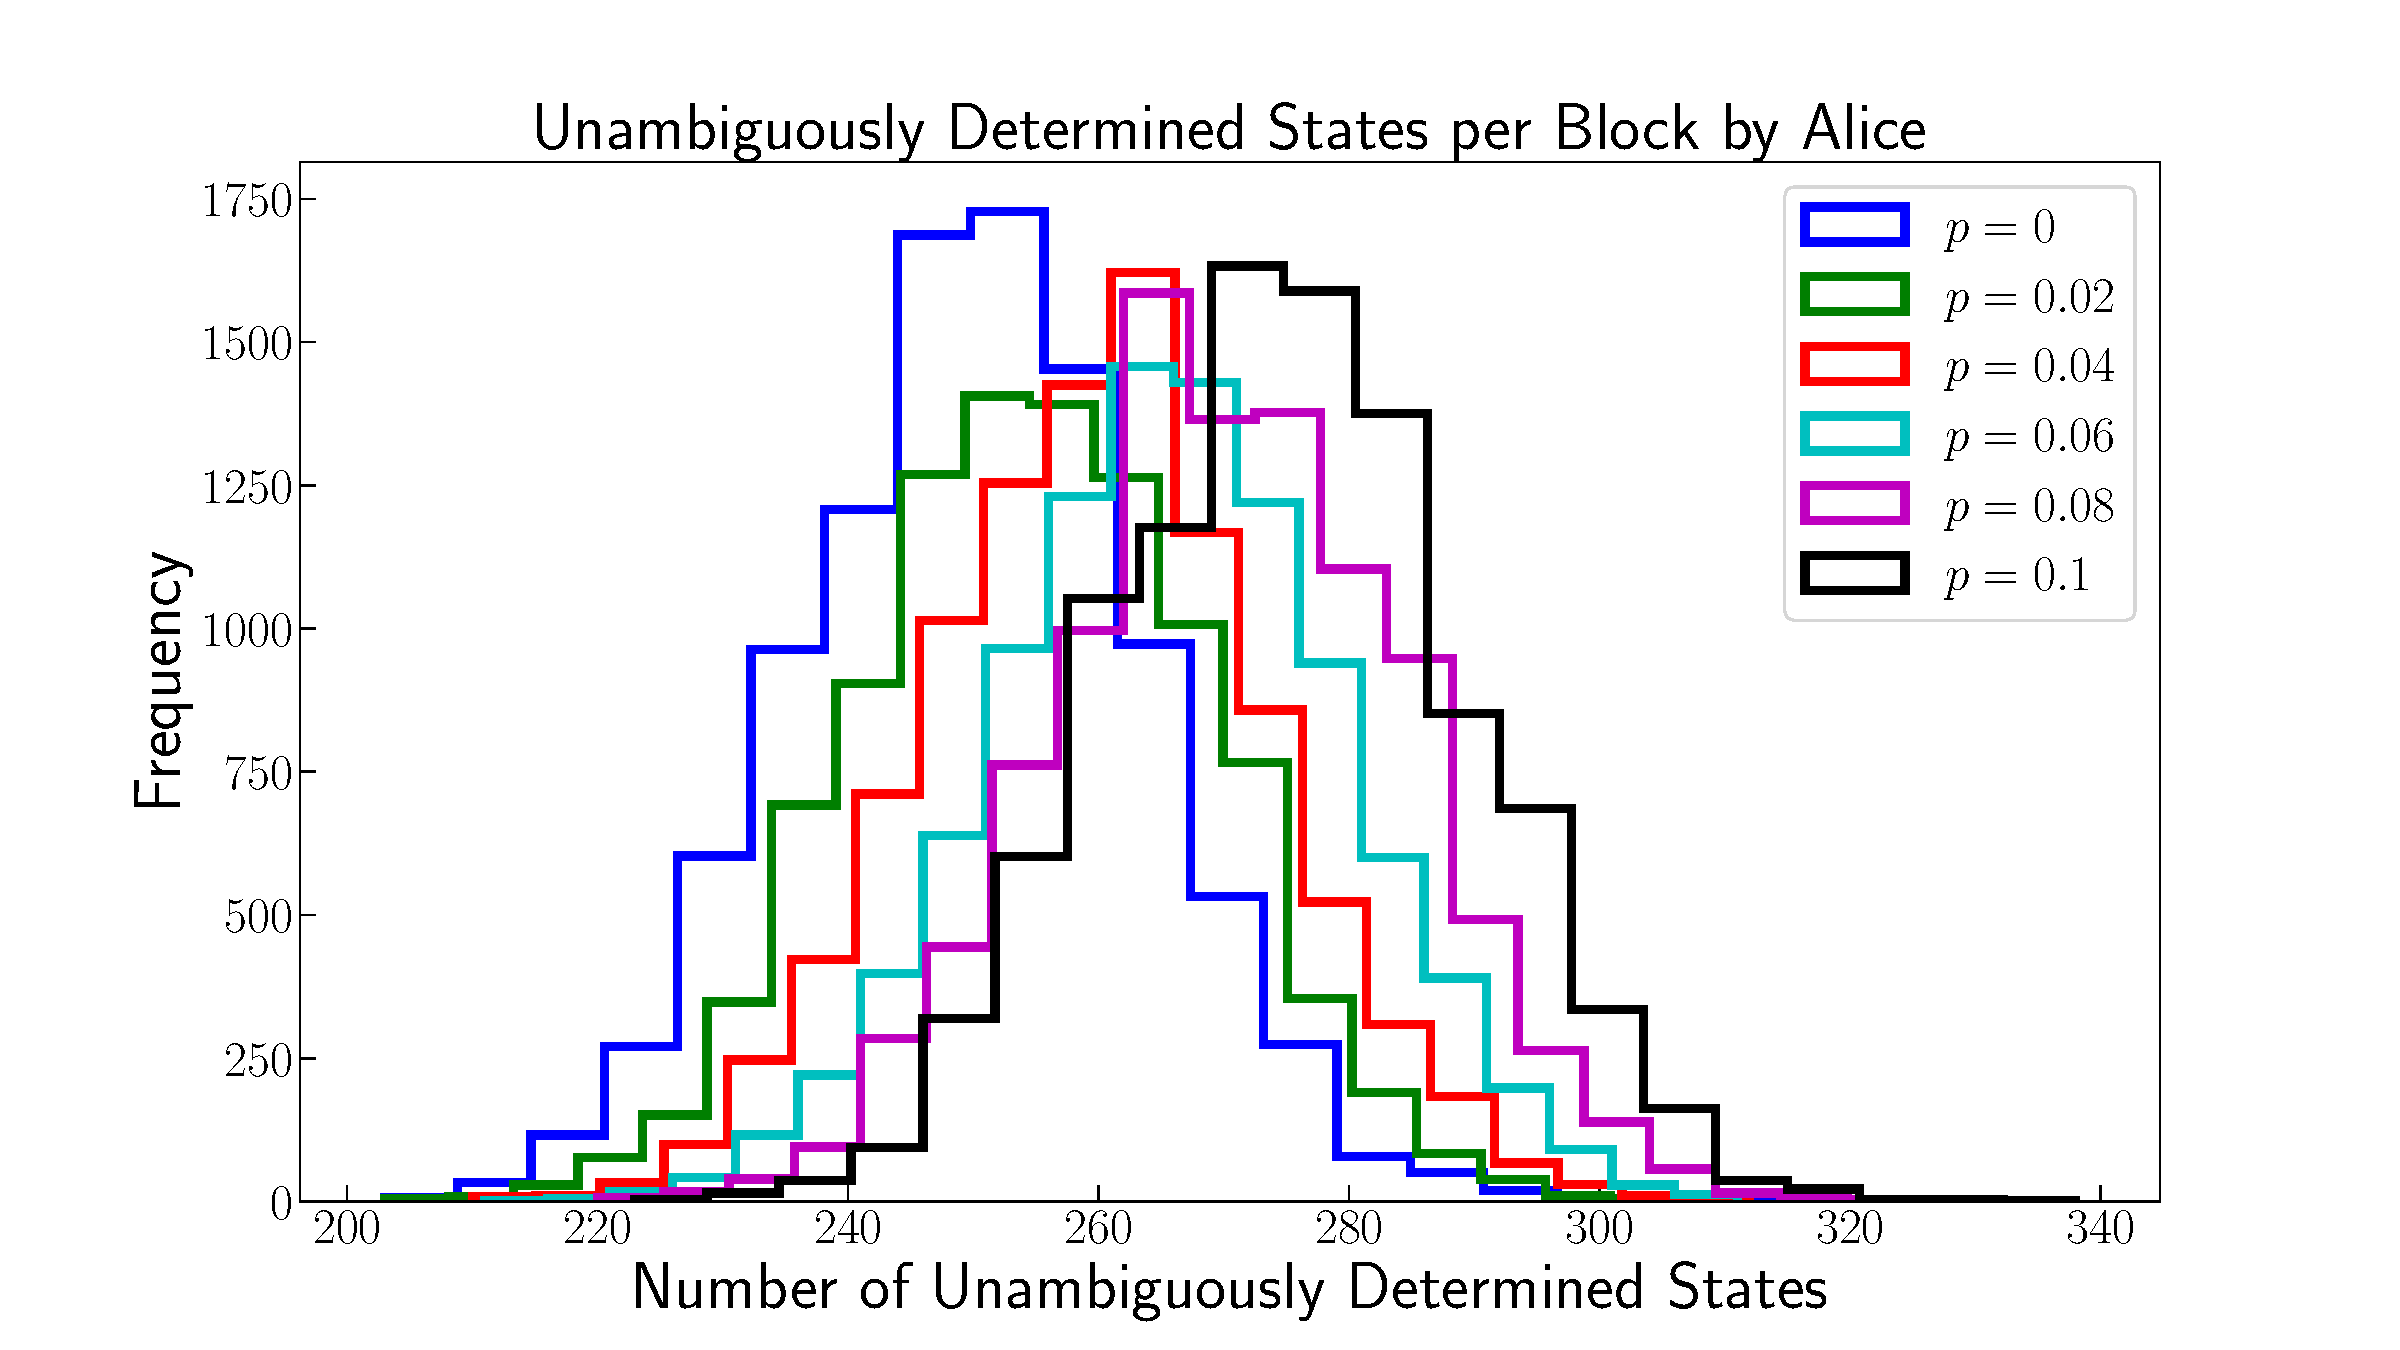
\includegraphics[width=\linewidth]{USD_number_per_block_histogram_depolar.pdf}
    \caption{The histogram showing the number of unambiguously determined states by Bob for a typical run, for $n=10000, k=1000$ with different depolarizing noise $p=\{0, 0.02, 0.04, 0.06, 0.08, 0.10\}$.}
    \label{fig:USD_number_per_block_histogram}
\end{figure}
In Figure~\ref{fig:USD_number_per_block_histogram}, it shows the histogram shows the number of unambiguously determined states by Bob, for $n=10000, k=1000$ with depolarizing noise range from $p=\{0, 0.02, 0.04, 0.06, 0.08, 0.10\}$. When $p=0$, we can clearly see that the histogram peaks at around $250$, which means, most of the blocks have around $1/4$ of the states being unambiguously determined. And the peak of the number of unambiguously determined states shifts to the right when we introduced noise in the simulation, the analysis is in Appendix~\ref{sec:Depolarizing_and_Dephasing_Noise}. 

Regardless of the noise level, the number of unambiguously determined states per block follows a Gaussian distribution, where the probability of a block with $x$ unambiguously determined states decreases exponentially with $x$ when $x$ is large. This gives the asymptotic security against Bob cheating of our protocol.

\begin{figure}
    \centering
    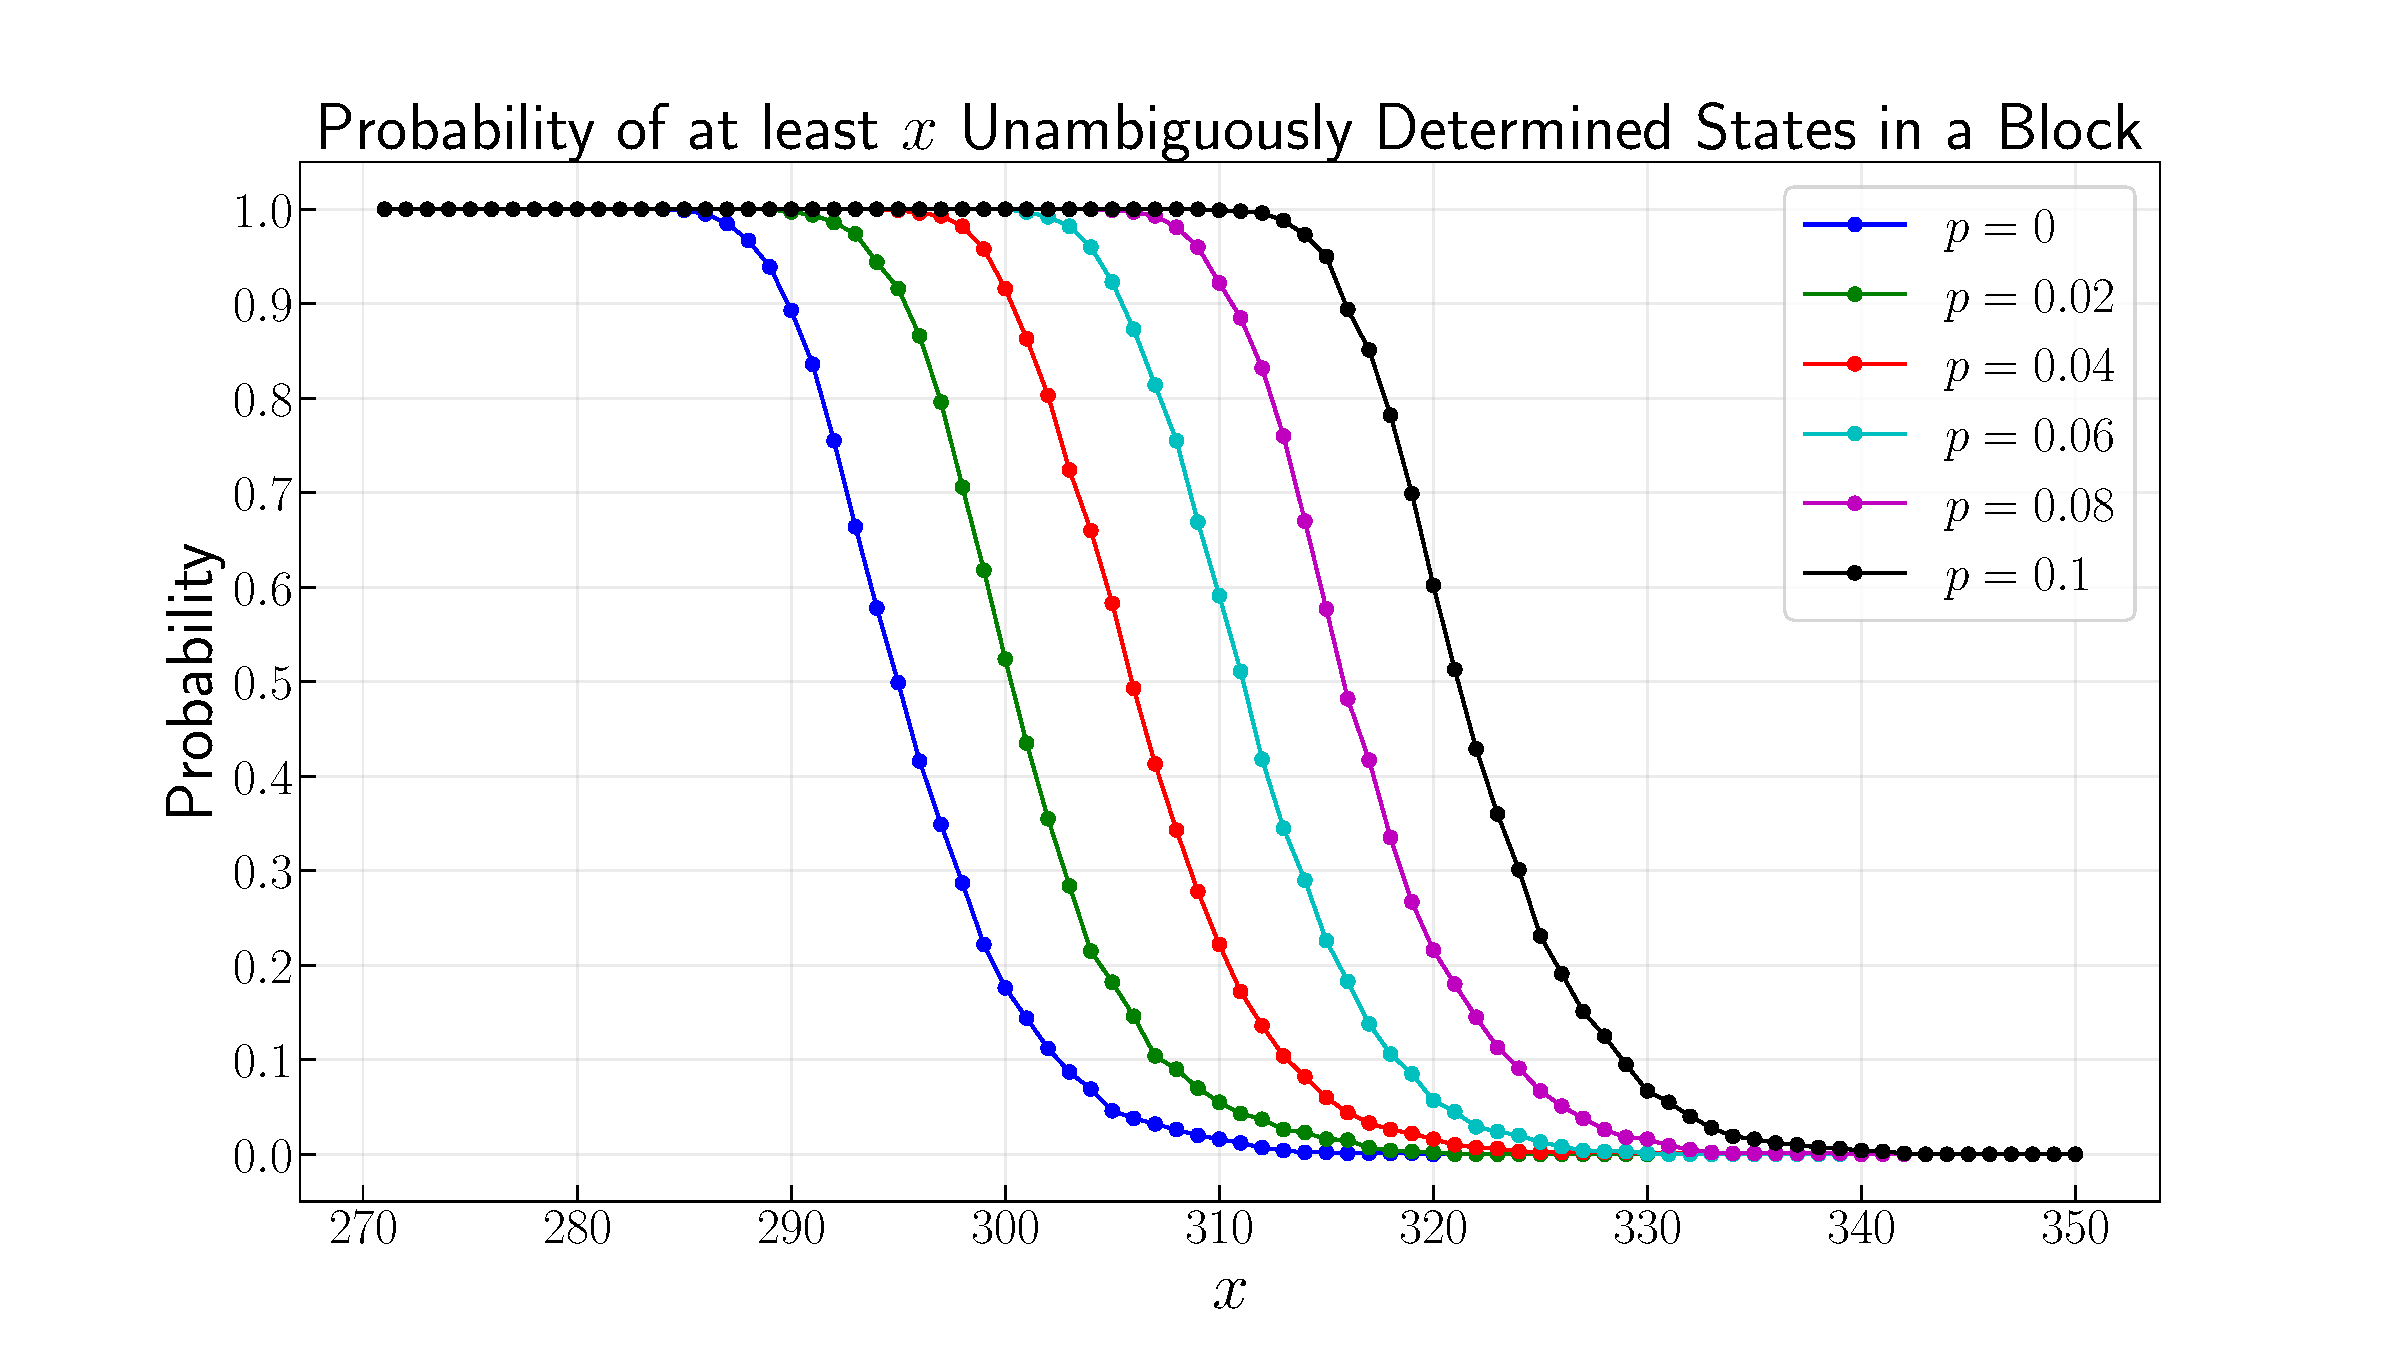
\includegraphics[width=\linewidth]{Probability_at_least_x_USD_states_depolar.pdf}
    \caption{The probability of at least $x$ unambiguously determined state in a block, calculated by running $1000$ times of simulation for $n=1000, k=1000$ with different depolarizing noise $p=\{0, 0.02, 0.04, 0.06, 0.08, 0.10\}$. The figure is chopped between $x\in[270, 350]$, because $p=1$ for all $x<270$ and $p=0$ for all $x>350$.}
    \label{fig:Probability_at_least_x_USD_states}
\end{figure}

Figure~\ref{fig:Probability_at_least_x_USD_states} shows the probability of at least $x$ unambiguously determined state in a block, calculated by running $1000$ times of simulation for $n=1000, k=1000$ and with different depolarizing noise $p=\{0, 0.02, 0.04, 0.06, 0.08, 0.10\}$, the figure only shows $x\in[270, 350]$ because $p=1$ for all $x<270$ and $p=0$ for all $x>350$. 

In the noiseless case, we can see that the probability dropped exponentially at the threshold value around $290$. And with the presence of noise, the probability still dropped exponentially, while the threshold value shifted to the right. Thus, when Alice and Bob have estimated the noise in the channel, Alice can choose a QECC with some finite distance, to make sure that the probability of Bob getting more information vanish asymptotically.

\section{Conclusion}

This paper proposes a one-way, prepare-and-measure quantum protocol intended to realize symmetric private information retrieval (SPIR) between a single client and a single classical database, providing statistical security guarantees. Where the client requests specific data from a database, we propose a scheme to achieve this without leaking extra information to the client, while keeping the client's interested bits secure to the database.

In particular, the construction combines QKD-style transmission phase (to ensure security against eavesdropping), unambiguous state discrimination (to create client-side asymmetry in which bits are known), and a random blocking with QECC post-processing step that aims to ensure the client can decode essentially only one requested item while learning asymptotically negligible additional database information, together with explicit parameter trade-offs and an overhead bound.

Security against an all-powerful eavesdropper is obtained by adopting standard QKD steps (parameter estimation, reconciliation, and privacy amplification) to bound the adversary's information, and by reusing a portion of the generated secret key as a resource in later post-processing. Client's privacy is supported by the fact that the server cannot reliably determine which signals were unambiguously identified by the client.

The analysis makes explicit the trade-offs among database size $n$, block size $k$, USD success probability $b$, channel error rate $e$, and an additional overhead $h$ required to enable suitable coding, including a stated lower bound on $h$ in terms of these parameters and the QKD threshold error rate. 

In the simulation, we have shown that with and without noise, the database can unambiguously determine a certain number of bits in each block, and the number of unambiguously determined states follows a Gaussian distribution with a shifted mean. We showed that by selecting an appropriate threshold for the QECC, the database can ensure the client gains asymptotically no information on other bits.

In summary, we proposed the first single-database quantum SPIR with information-theoretic aspirations with only one-way quantum communication. We give the candidate protocol that uses only one-way quantum communication and standard BB84/QKD-style prepare-and-measure components rather than assuming multiple non-colluding servers or computational assumptions in previous experimental realizations~\cite{QSPIR_multiple_database1, QSPIR_multiple_database2, QSPIR_theory1}. Our candidate protocol is easily implementable with the current BB84-style QKD experimental setups, which have a great impact on quantum cryptography and the information acquisition processes. For instance, our protocol will be beneficial in applications like official investigations, and this protocol enhances our understanding of the limits of quantum cryptography.



\appendix

\section{Review on QKD Security}
\label{sec:Review_qkd_security}
In this section, we will briefly review the security proof of QKD, including the Shor-Preskill security proof and the threshold key rates~\cite{Shor_Preskill_Proof1}. Subsequently, we will review the corrections on key rates needed when dealing with finite-key analysis. 

Many previous results have proven the security of QKD, for example, as proven by Lo and Chau~\cite{Lo_Chau_proof}, Shor, and Preskill~\cite{Shor_Preskill_Proof1}.

Specifically, in Shor and Preskill's framework of the BB84 QKD protocol, they have proven that a CSS-based entanglement-distillation protocol (a QEC procedure) is operationally equivalent to a prepare-and-measure scheme with classical information reconciliation followed by privacy amplification to extract a shared private key~\cite{Shor_Preskill_Proof1}. And the Shor-Preskill key rate is given by,
\begin{equation}
    R\le 1-H(e_b)-H(e_p)
\end{equation}
where $e_b$ and $e_p$ represents the bit-flip and phase-flip error, and $H(x)=-x\log_2x-(1-x)\log_2(1-x)$ is the binary entropy function. If we assume that $e_b=e_p$, the equation can be further reduced to
\begin{equation}
    R \le 1-2H(e)
\end{equation}
where $e$ is the qubit error rate~\cite{Shor_Preskill_Proof1}. It is easy to show that the threshold error rate for $R>0$ is

\begin{equation}
\begin{split}
    H(e_{thr})&<1/2\\
    e_{thr}&\lessapprox 11\%
\end{split}
\end{equation}

Here we state a walking theorem; later in Section~\ref{sec:Bob_Cheating}, we will present the full theorem with a proof.

\begin{theorem}
    For any channel qubit error rate $e<e_{thr}$, where $e_{thr}$ is the threshold qubit error rate of the QKD protocol used, the presented SPIR protocol in Section~\ref{sec:the_protocol} can be achieved with some overhead of $h$.
\label{thm:walking_theorem}
\end{theorem}
Notice that the above bounds works for asymptotic case with an infinite key length. In more realistic settings, one has to consider the finite key analysis.

\subsection{Review on Finite Key Analysis for QKD}
\label{sec:Finite_key_analysis_qkd}
The analysis presented above establishes bounds that are attained in the asymptotic limits, and in reality, Alice and Bob can never share an infinitely long qubit string. Therefore, in this subsection, we present the finite-key analysis of our protocol, which incorporates corrections to the asymptotic bounds. We will demonstrate the correction needed for our protocol under the finite-key effect.

The finite key analysis has been well-explored in both the discrete and continuous variable QKD settings, inspired by the well-developed classical algorithms, for example, Ref.~\cite{Finite_key_analysis1, Finite_key_analysis2, Finite_key_analysis3, Rates_for_realistic_code1, Rates_for_realistic_code2, Rates_for_realistic_code3}. Ref.~\cite{Rates_for_realistic_code2} gives a nice review on different QKD schemes, possible side channel attacks, and how to save them with proper realistic code key rates. Since the SPIR scheme presented in this paper is backed by QKD, most of the finite-key analysis bounds proven in previous literature apply to our protocol. 

In this subsection, we review the main idea and bounds from the finite-key analysis on discrete variable QKD proven in Ref.~\cite{Finite_key_analysis1}, as the bounds proven are relatively tight and fit for theoretical settings.

A realistic QKD protocol is defined by a six-tuple, (notice that the parameters introduced in this subsection may carry different meanings as the parameters in our protocol) $\Phi[n, m, l, e_{tol}, \epsilon_{cor}, \text{leak}_{EC}]$, where $n$ is the size of raw keys, $m$ is the number of bits used for parameter estimation, $l$ is the final shared private key length, $e_{tol}$ is the channel error tolerance, $\epsilon_{cor}$ is the required correctness, which is defined as $\text{Pr}[\mathbf{S_{A}}\ne \mathbf{S_{B}}]\le\epsilon_{cor}$; and finally the error correction leakage $\text{leak}_{EC}$.

Also, Ref.~\cite{Finite_key_analysis1} defines another quantity $q$, named as ``preparation quality'', which is defined as the maximum fidelity between states prepared in the $X$ basis $\psi_X$ and states prepared in the $Z$ basis $\psi_Z$.
\begin{equation}
    q=-\log_2\max|\bra{\psi_X}\ket{\psi_Z}|^2
\end{equation}

If the states are prepared in a perfect $X$ basis or $Z$ basis, then $q=1$. With all the definitions, the finite-key analysis has shown that a protocol $\Phi[n, m, l, e_{tol}, \epsilon_{cor}, \text{leak}_{EC}]$ using a source with  preparation quality $q$ that is $\epsilon_{sec}$-secret if the secret key length $l$ satisfies~\cite{Finite_key_analysis1}:
\begin{equation}
    l\le n(q-H(e_{tol}+\mu))-\text{leak}_{EC}-\log_2 \frac{2}{\epsilon_{sec}^2\epsilon_{cor}}
    \label{eq:realistic_l}
\end{equation}
where $\mu$ is the term which accounts for statistical fluctuations, that
\begin{equation}
    \mu := \sqrt{\frac{n+m}{nm}\frac{m+1}{m}\ln\frac{2}{\epsilon_{sec}}}
\end{equation}

Usually, $\text{leak}_{EC}$ is taken to be about $1.16nH(e_{tol})$ to specify the ``inefficiency ratio'' of the actual error correction code used~\cite{Finite_key_analysis1}. Then, we can define the finite-key rate with QKD protocol $\Phi$ and channel error rate $Q$ in the case as
\begin{equation}
    r_{real}(\Phi, Q) =\frac{l}{M(n, m)}
\end{equation}
Where $M(n, m)$ is the expected number of qubits that need to be exchanged until $n$ raw key bits and $m$ bits for parameter estimation are gathered.

Here, let us make the assumption that $\frac{1}{M(n, m)}=\frac{1}{cn}$ for some not too big constant $c$. Then, we can rewrite the finite key-rate by plugging in the $l$ in equation~\ref{eq:realistic_l}, we obtain:

\begin{equation}
\begin{split}
    r_{real}&\approx (q-H(e_{tol}+\mu)-1.16H(e_{tol}))/c-\frac{\log_2 \frac{2}{\epsilon_{sec}^2\epsilon_{cor}}}{nc}\\
    &= q-H(e_{tol}+\mu)-1.16H(e_{tol}))/c-r_{cor}
    \end{split}
    \label{eq:realistic_rate}
\end{equation}

In equation~\ref{eq:realistic_rate}, the first term is almost identical to the key rate at asymptotic limits, where the second term can be thought of as a finite-key rate correction $r_{cor}$.


\section{Depolarizing and Dephasing Noise}
\label{sec:Depolarizing_and_Dephasing_Noise}

A quantum channel can be described by a CPTP map, which can be written in many different representations. For example, in the Kraus representation, a channel on a state $\rho$, $\mathcal{E}(\rho)$, can be written as:
\begin{equation}
    \mathcal{E}(\rho)=\sum_K \lambda_K K^\dagger\rho K
\end{equation}
where $K$ is called the Kraus operators, which satisfy 
\begin{equation}
    \sum_KK^\dagger K=I
\end{equation}
and the parameters $\lambda_K>0$.
Here, we consider the two most common types of errors, the depolarizing noise and the dephasing noise, and we explore their effect on the error rate of USD.

Recall that for a state $\rho$ and an projective operator $P$, the probability of projecting $\rho$ onto $P$ is given by
\begin{equation}
    p_{projection}(\rho, P)=Tr[\rho P]
\end{equation}

\subsection{Depolarizing Noise}
The general form of depolarizing noise with depolarizing probability $p$ on a $d$-level quantum system in Kraus representation is:
\begin{equation}
    \mathcal{E}^{depolar}_{p}(\rho)=(1-p)\rho+p\frac{I}{d}
\end{equation}

Here, we consider 2-level systems without generalized measurement. We can easily check that if a state $\rho$ is originally prepared in either $\sigma_X$ or $\sigma_Z$ basis, then the state undergoes depolarization, and being measured in the complementary basis, the probability of getting either result is still $1/2$. Mathematically, 
\begin{equation}
    Tr[\mathcal{E}^{depolar}_p(\rho_0)P]=1/2
\end{equation}
for all the following combinations: $(\rho_0, P)=(\ket{0\text{ or }1}\bra{0\text{ or }1}, \ket{\pm}\bra{\pm}), (\ket{\pm}\bra{\pm}, (\ket{0\text{ or }1}\bra{0\text{ or }1})$.

Hence, if Alice prepares a state and sends it to Bob under a depolarizing channel, the probability of correctly USD is not changed. What does change is the false positive rate. For example, if Alice prepares the state $\ket{0}$, and Bob measures in $\sigma_Z$ basis and gets $\ket{1}$.

\begin{equation}
Tr[\mathcal{E}^{depolar}_p(\ket{0}\bra{0})\ket{1}\bra{1}]=p/2
\end{equation}

Which means, when Alice prepares state $\ket{0}$, and Bob measures in $\sigma_Z$, with probability $p/2$, Bob will obtain the state $\ket{1}$. Denotes $\ket{\psi}_B$ as the initial state prepared by Alice, $P_A$ as the measurement basis chosen by Bob, and $r_A\in\{+1, -1\}$ as the measurement result. This error happened to the 4 cases, $\left(\ket{\psi}_B, P_A, r_A\right)=(\ket{0},\sigma_Z, -1), (\ket{1},\sigma_Z, +1), (\ket{+},\sigma_X, -1), (\ket{-},\sigma_X, +1)$. Each of the 4 cases happens with probability $p/2$ upon the chosen of specific basis.

Hence, the probability of a state measurement being falsely considered as a successful USD:
\begin{equation}
    \text{False Positive}=\frac{1}{4}\times\frac{1}{2}\times\frac{p}{2}\times4 = \frac{p}{4}
\end{equation}

Hence, the False positive error rate:
\begin{equation}
    e_{depolar}=\frac{p/4}{1/4+p/4}=\frac{p}{1+p}
\end{equation}

\subsection{Dephasing Noise}
The general form of dephasing noise with dephasing probability in $\sigma_X$, $\sigma_Y$ and $\sigma_Z$ direction with probability $p_X, p_Y, p_Z$ on a $d$-level quantum system in Kraus representation is:
\begin{equation}
    \mathcal{E}^{dephase}_{p_x, p_y, p_z}(\rho)=(1-p_x-p_y-p_Z)\rho+\sum_{D=X, Y, Z}p_D\sigma_D\rho\sigma_D^\dagger
\end{equation}

We can easily check that if a state $\rho$ is original prepared in either $\sigma_X$ or $\sigma_Z$ basis, then the state undergoes dephasing of arbitrary noise, and being measured in the complementary basis, the probability of getting either results are still $1/2$.
\begin{equation}
    Tr[\mathcal{E}^{dephase}_{p_x, p_y, p_z}(\rho_0)P]=1/2
\end{equation}
for all the following combinations: $(\rho_0, P)=(\ket{0\text{ or }1}\bra{0\text{ or }1}, \ket{\pm}\bra{\pm}), (\ket{\pm}\bra{\pm}, (\ket{0\text{ or }1}\bra{0\text{ or }1})$.

Hence, if Alice prepares a state and sends to Bob under a dephasing channel, the probability of correctly USD is not changed. What does change is the false positive rate, For example, if Alice prepares state $\ket{0}$, and Bob measures in $\sigma_Z$ basis and gets $\ket{1}$.
\begin{equation}
Tr[\mathcal{E}^{dephase}_{p_x, p_y, p_z}(\ket{0}\bra{0})\ket{1}\bra{1}]=p_x+p_y
\end{equation}
\begin{equation}
Tr[\mathcal{E}^{dephase}_{p_x, p_y, p_z}(\ket{1}\bra{1})\ket{0}\bra{0}]=p_x+p_y
\end{equation}
\begin{equation}
Tr[\mathcal{E}^{dephase}_{p_x, p_y, p_z}(\ket{+}\bra{+})\ket{-}\bra{-}]=p_y+p_z
\end{equation}
\begin{equation}
Tr[\mathcal{E}^{dephase}_{p_x, p_y, p_z}(\ket{-}\bra{-})\ket{+}\bra{+}]=p_y+p_z
\end{equation}

Hence, the probability of a state measurement being falsely considered as a successful USD:
\begin{equation}
\begin{split}
    \text{False Positive}&=\frac{1}{4}\times\frac{1}{2}\times\left(2p_x+2p_y+2p_y+2p_z\right)\\
    &=\frac{p_x+2p_y+p_z}{4}
    \end{split}
\end{equation}

Hence, the False positive error rate:
\begin{equation}
    e_{depolar}=\frac{\frac{p_x+2p_y+p_z}{4}}{1/4+\frac{p_x+2p_y+p_z}{4}}=\frac{p_x+2p_y+p_z}{1+p_x+2p_y+p_z}
\end{equation}

\section{Collective USD Does Not Provide Improvement}

One curious question is: in our main protocol, Alice sends the qubits to Bob, and Bob performs USD one by one. One may wonder: if, instead of doing it successively, Bob does a collective USD on multiple received qubits, will it provide any advantages over? The answer is no. This is proven in much of the literature, for example, Ref.~\cite{USD_one_by_one}.



\bibliography{SPIR_Single_Database}% Produces the bibliography via BibTeX.

\end{document}
%
% ****** End of file apssamp.tex ******
